% Options for packages loaded elsewhere
\PassOptionsToPackage{unicode}{hyperref}
\PassOptionsToPackage{hyphens}{url}
%
\documentclass[
  12pt,
  letterpaper]{article}
\usepackage{lmodern}
\usepackage{amssymb,amsmath}
\usepackage{ifxetex,ifluatex}
\ifnum 0\ifxetex 1\fi\ifluatex 1\fi=0 % if pdftex
  \usepackage[T1]{fontenc}
  \usepackage[utf8]{inputenc}
  \usepackage{textcomp} % provide euro and other symbols
\else % if luatex or xetex
  \usepackage{unicode-math}
  \defaultfontfeatures{Scale=MatchLowercase}
  \defaultfontfeatures[\rmfamily]{Ligatures=TeX,Scale=1}
\fi
% Use upquote if available, for straight quotes in verbatim environments
\IfFileExists{upquote.sty}{\usepackage{upquote}}{}
\IfFileExists{microtype.sty}{% use microtype if available
  \usepackage[]{microtype}
  \UseMicrotypeSet[protrusion]{basicmath} % disable protrusion for tt fonts
}{}
\usepackage{xcolor}
\IfFileExists{xurl.sty}{\usepackage{xurl}}{} % add URL line breaks if available
\IfFileExists{bookmark.sty}{\usepackage{bookmark}}{\usepackage{hyperref}}
\hypersetup{
  pdftitle={The locally Gaussian partial correlation},
  pdfauthor={Håkon Otneim and Dag Tjøstheim},
  hidelinks,
  pdfcreator={LaTeX via pandoc}}
\urlstyle{same} % disable monospaced font for URLs
\usepackage[margin = 1in]{geometry}
\usepackage{longtable,booktabs}
% Correct order of tables after \paragraph or \subparagraph
\usepackage{etoolbox}
\makeatletter
\patchcmd\longtable{\par}{\if@noskipsec\mbox{}\fi\par}{}{}
\makeatother
% Allow footnotes in longtable head/foot
\IfFileExists{footnotehyper.sty}{\usepackage{footnotehyper}}{\usepackage{footnote}}
\makesavenoteenv{longtable}
\usepackage{graphicx}
\makeatletter
\def\maxwidth{\ifdim\Gin@nat@width>\linewidth\linewidth\else\Gin@nat@width\fi}
\def\maxheight{\ifdim\Gin@nat@height>\textheight\textheight\else\Gin@nat@height\fi}
\makeatother
% Scale images if necessary, so that they will not overflow the page
% margins by default, and it is still possible to overwrite the defaults
% using explicit options in \includegraphics[width, height, ...]{}
\setkeys{Gin}{width=\maxwidth,height=\maxheight,keepaspectratio}
% Set default figure placement to htbp
\makeatletter
\def\fps@figure{htbp}
\makeatother
\setlength{\emergencystretch}{3em} % prevent overfull lines
\providecommand{\tightlist}{%
  \setlength{\itemsep}{0pt}\setlength{\parskip}{0pt}}
\setcounter{secnumdepth}{5}
\usepackage{setspace}
\usepackage{sectsty}
\usepackage{graphicx}
\usepackage{subfig}
\usepackage{bm}

\doublespacing
\sectionfont{\centering}

\newcommand{\X}{\bm{X}}
\newcommand{\Xone}{\bm{X}^{(1)}}
\newcommand{\Xtwo}{\bm{X}^{(2)}}
\newcommand{\xtwo}{\bm{x}^{(2)}}
\newcommand{\x}{\bm{x}}
\newcommand{\hX}{\widehat{X}}
\newcommand{\tX}{\tilde{X}}

\newcommand{\Z}{\bm{Z}}
\newcommand{\z}{\bm{z}}
\newcommand{\hz}{\widehat{z}}
\newcommand{\hfz}{\widehat{\bm{z}}}
\newcommand{\hZ}{\widehat{\bm{Z}}}
\newcommand{\hnZ}{\widehat{Z}}
\newcommand{\Zone}{\bm{Z}^{(1)}}
\newcommand{\Ztwo}{\bm{Z}^{(2)}}
\newcommand{\zone}{\bm{z}^{(1)}}
\newcommand{\ztwo}{\bm{z}^{(2)}}

\newcommand{\D}{\bm{D}}
\newcommand{\hD}{\widehat{\bm{D}}}

\newcommand{\y}{\bm{y}}
\newcommand{\Y}{\bm{Y}}
\newcommand{\hY}{\widehat{Y}}

\newcommand{\fv}{\bm{v}}
\newcommand{\fu}{\bm{u}}

\newcommand{\fC}{\bm{C}}
\newcommand{\fA}{\bm{A}}
\newcommand{\fV}{\bm{V}}
\newcommand{\M}{\bm{M}}
\newcommand{\J}{\bm{J}}

\newcommand{\R}{\bm{R}}
\newcommand{\hR}{\widehat{\bm{R}}}

\newcommand{\hF}{\widehat{F}}
\newcommand{\hf}{\widehat{f}}

\newcommand{\hrho}{\widehat{\rho}}
\newcommand{\frho}{\bm{\rho}}
\newcommand{\hfrho}{\widehat{\bm{\rho}}}

\newcommand{\hh}{\bm{b}}
\newcommand{\bb}{\bm{b}}

\newcommand{\fmu}{\bm{\mu}}
\newcommand{\hfmu}{\widehat{\bm{\mu}}}
\newcommand{\hsigma}{\widehat{\sigma}}
\newcommand{\fSigma}{\bm{\Sigma}}
\newcommand{\hfSigma}{\widehat{\bm{\Sigma}}}
\newcommand{\halpha}{\widehat{\alpha}}
\newcommand{\falpha}{\bm{\alpha}}
\newcommand{\hfalpha}{\widehat{\bm{\alpha}}}
\newcommand{\fOmega}{\bm{\Omega}}
\newcommand{\fLambda}{\bm{\Lambda}}
\newcommand{\fepsilon}{\bm{\epsilon}}

\newcommand{\Jb}{\bm{J}_{\hh}}
\newcommand{\Mb}{\bm{M}_{\hh}}

\newcommand{\Cov}{\textrm{Cov}}
\newcommand{\E}{\textrm{E}}
\newcommand{\Var}{\textrm{Var}} 
\newcommand{\di}{\,\textrm{d}}
\newcommand{\Corr}{\textrm{Corr}} 



\usepackage{color}
\usepackage{colortbl}

\definecolor{Gray}{gray}{0.9}
\newlength{\cslhangindent}
\setlength{\cslhangindent}{1.5em}
\newenvironment{cslreferences}%
  {\setlength{\parindent}{0pt}%
  \everypar{\setlength{\hangindent}{\cslhangindent}}\ignorespaces}%
  {\par}

\title{The locally Gaussian partial correlation}
\author{Håkon Otneim\footnote{Corresponding author. Department of Business and Management Science, NHH Norwegian School of Economics. Helleveien 30, 5045 Bergen, Norway. \texttt{hakon.otneim@nhh.no}} and Dag Tjøstheim\footnote{University of Bergen \newline {Acknowledgements:} The authors gratefully acknowledge the input of an associate editor as well as two anonymous referees, whose comments have greatly improved this paper.}}
\date{}

\usepackage{amsthm}
\newtheorem{theorem}{Theorem}[section]
\newtheorem{lemma}{Lemma}[section]
\newtheorem{corollary}{Corollary}[section]
\newtheorem{proposition}{Proposition}[section]
\newtheorem{conjecture}{Conjecture}[section]
\theoremstyle{definition}
\newtheorem{definition}{Definition}[section]
\theoremstyle{definition}
\newtheorem{example}{Example}[section]
\theoremstyle{definition}
\newtheorem{exercise}{Exercise}[section]
\theoremstyle{remark}
\newtheorem*{remark}{Remark}
\newtheorem*{solution}{Solution}
\let\BeginKnitrBlock\begin \let\EndKnitrBlock\end
\begin{document}
\maketitle
\begin{abstract}
It is well known in econometrics and other fields that the dependence structure for jointly Gaussian variables can be fully captured using correlations, and that the \textit{conditional} dependence structure in the same way can be described using partial correlations. The partial correlation does not, however, characterize conditional dependence in many non-Gaussian populations. This paper introduces the local Gaussian partial correlation (LGPC), a new measure of conditional dependence. It is a local version of the partial correlation coefficient that characterizes conditional dependence in a large class of populations. It has some useful and novel properties besides: The LGPC reduces to the ordinary partial correlation for jointly normal variables, and it distinguishes between positive and negative conditional dependence. Furthermore, the LGPC can be used to study departures from conditional independence in specific parts of the distribution. We provide several examples of this, both simulated and real, and derive estimation theory under a local likelihood estimation framework. Finally, we indicate how the LGPC can be used to construct a powerful test for conditional independence, which, for example, can be used to detect nonlinear Granger causality in time series. \newline \textbf{Keywords:} \emph{Conditional dependence, conditional independence test, Granger causality}
\end{abstract}

\hypertarget{introduction}{%
\section{INTRODUCTION}\label{introduction}}

Estimation of conditional dependence and testing for conditional independence are important topics in classical as well as modern statistics. In the last two decades, for instance, there have been intense developments in using conditional dependence for probabilistic networks, conditional multivariate time series analysis as well as copula analysis. For jointly Gaussian variables, conditional dependence is measured by the partial correlation coefficient. Given three jointly Gaussian stochastic variables \(X_1\), \(X_2\) and \(X_3\), \(X_1\) and \(X_2\) are conditionally independent given \(X_3\) if and only if the partial correlation between \(X_1\) and \(X_2\) given \(X_3\) is equal to zero. There is a rich literature on applications of the partial correlation coefficient to Gaussian networks, path analysis and causality. The Gaussian assumption is strict, however, and it is easy to find non-Gaussian examples where the partial correlation function completely fails in describing conditional dependence, as will be seen later in this article.

The purpose of this paper is to introduce a new concept for measuring conditional dependence. This concept retains all the properties of the ordinary partial correlation in the Gaussian case, but seeks to avoid the weaknesses of this measure in the non-Gaussian case. This is done by fitting a \emph{family} of Gaussian distributions to a given continuous multivariate distribution and exploiting the simple conditioning rules of the Gaussian distribution \emph{locally}. This approach produces a new measure of conditional dependence, \emph{the local Gaussian partial correlation (LGPC)} which, being directly related to the ordinary partial correlation, is easy to interpret, and reduces to the very same ordinary partial correlation in the Gaussian case. Moreover, it distinguishes between positive and negative conditional dependence whereas competing non-linear measures report only the \emph{strength} of the conditional dependence on some non-negative scale.

The local view gives much more flexibility. It allows the conditional dependence to be stronger or weaker in certain regions of a multivariate distribution than in others. This is of particular interest in finance, where description of tail behavior is important. The local aspect also makes it possible to focus tests of conditional independence to selected parts of the distribution, which may potentially increase the power of the test.

The local approach has been shown to be advantageous in other areas of statistics, such as the measurement of nonlinear dependence, density estimation and spectral analysis, see for instance Tjøstheim and Hufthammer (\protect\hyperlink{ref-tjostheim2013local}{2013}), Otneim and Tjøstheim (\protect\hyperlink{ref-otneim2017locally}{2017}) and Jordanger and Tjøstheim (\protect\hyperlink{ref-jordanger2017nonlinear}{2020}). The present paper, then, represents the first attempt to model conditional dependence locally. There are several other approaches to modelling conditional dependence and testing for conditional independence in the non-Gaussian case in the literature. For the most part, they revolve around test statistics in conditional independence tests. Such statistics are usually based on measures of distance between some property of the sample and the corresponding property of the population under the null hypothesis of conditional independence. As a consequence, the conditional dependence measures are not always easy to interpret, and can, as mentioned above, not distinguish between negative and positive conditional dependence. We present a comprehensive set of references to this literature in Section \ref{chap:testing}.

Definitions and properties are presented in Section \ref{chap:conditional}, whereas estimation is covered in Section \ref{chap:estimation}. Two examples illustrating the strengths of our approach are given in Section \ref{chap:example}. Section \ref{chap:testing} gives a brief account of the potential in testing.

An integral part of our article is the online supplement. It deals with a number of issues complementing the treatment in the main paper. Among them are more examples, extensions of the main concept to more general situations, precise formulations of some theoretical results with proofs, as well as discussions of local asymptotic power and the Pitman criterion for testing, and validity of the use of the bootstrap.

\hypertarget{chap:conditional}{%
\section{THE LOCAL GAUSSIAN PARTIAL CORRELATION}\label{chap:conditional}}

Let \(\X = (X_1, \ldots, X_p)\) be a random vector. Denote by \((\X_1,\X_2,\X_3)\) a partition of \(\X\) into vectors of dimension \(d_1\), \(d_2\) and \(d_3\) respectively, such that \(\Xone = (\X_1, \X_2) = (X_1, \ldots,X_{d_1 + d_2})\) consists of the first \(d_1+d_2\) components in \(\X\) and \(\Xtwo = \X_3 = (X_{d_1+d_2+1}, \ldots, X_{d_1+d_2+d_3})\) contains the remaining \(d_3\) variables, where \(p = d_1+d_2+d_3\). We assume that the mean vector \(\fmu\) and covariance matrix \(\fSigma\) of \(\X\) exist, and partition them correspondingly, writing
\begin{equation}
\fmu = \begin{pmatrix} \fmu_1 \\ \fmu_2 \\ \fmu_3 \end{pmatrix} \,\,\,\, \textrm{ and } \,\,\,\, \fSigma = \begin{pmatrix} \fSigma_{11} & \fSigma_{12} & \fSigma_{13} \\ \fSigma_{21} & \fSigma_{22} & \fSigma_{23} \\ \fSigma_{31} & \fSigma_{32} & \fSigma_{33}\end{pmatrix},
\label{eq:matrixpartition}
\end{equation}
where \(\fSigma_{ij}\) is the covariance matrices of \((\X_i, \X_j)\), \(i,j = 1,2,3\). There are two main concepts of correlation when \(\Xtwo = \X_3\) is given, the \emph{partial} and the \emph{conditional} correlation, and they coincide in several joint distributions, among them the Gaussian. See e.g.~Baba, Shibata, and Sibuya (\protect\hyperlink{ref-baba2004partial}{2004}) for details. We will use the partial correlation as a starting point when defining the LGPC. The partial variance-covariance matrix of \(\Xone = (\X_1, \X_2)\) given \(\Xtwo = \X_3\) is
\begin{equation}
\fSigma_{12|3} = \fSigma^{11} - \fSigma^{12}\left(\fSigma^{22}\right)^{-1}\fSigma^{21},
\label{eq:matrixpartial}
\end{equation}
where
\[\fSigma^{11} = \begin{pmatrix} \fSigma_{11} & \fSigma_{12} \\ \fSigma_{21} & \fSigma_{22} \end{pmatrix}, \,\, \fSigma^{12} = \begin{pmatrix} \fSigma_{13} \\ \fSigma_{23} \end{pmatrix}, \,\,\fSigma^{21} = \begin{pmatrix} \fSigma_{31} & \fSigma_{32} \end{pmatrix} \, \textrm{ and } \, \fSigma^{22} = \fSigma_{33},\]
and \(\fSigma_{12|3}\) is the covariance matrix in the conditional (Gaussian) distribution of \(\Xone\) given \(\X_3\) if \(\X\) is jointly normal. The partial correlation matrix between \(\X_1\) and \(\X_2\) given \(\X_3\) is naturally defined as

\begin{equation}
\R_{12|3} = \D^{-1/2}\fSigma_{12|3}\D^{-1/2},
\label{eq:partialcorrelation}
\end{equation}
where \(\D = \textrm{diag}(\fSigma_{12|3})\). We identify in the same way the partial correlation matrix \eqref{eq:partialcorrelation} with the correlation matrix in the conditional (Gaussian) distribution of \(\Xone\) given \(\Xtwo\) if \(\X\) is jointly normal. Equations \eqref{eq:matrixpartial} and \eqref{eq:partialcorrelation} will serve as the starting point for our definition of the \emph{local} partial correlation.

\hypertarget{chap:definition}{%
\subsection{Definition}\label{chap:definition}}

In all of the following we assume that the components of \(\X\) are continuous with joint density function \(f_{\X}\). Given a point \(\x\), we approximate \(f_{\X}\) in a neighborhood of \(\x\) by a multivariate Gaussian density

\begin{equation} 
\psi(\x, \fv) = \frac{1}{(2\pi)^{p/2}|\fSigma(\x)|^{1/2}} \exp \left\{-\frac{1}{2}(\fv - \fmu(\x))^T\fSigma^{-1}(\x)(\fv - \fmu(\x))\right\},
\label{eq:localgaussian}
\end{equation}
where \(\x = (x_1\ldots, x_p)\), \(\fmu(\x) = \{\mu_j(\x)\}\) and \(\fSigma(\x) = \{\sigma_{jk}(\x)\}\) for \(j,k=1,\ldots, p\). Moving to another point \(\y\), there is another (generally different) Gaussian approximation \(\psi(\y, \fv)\). In this way we approximate \(f_{\X}\) by a family of multivariate Gaussian densities defined by a set of smooth parameter functions \(\{\fmu(\x), \fSigma(\x)\}\), and if \(f_{\X}\) is itself a Gaussian density, then the parameter functions collapse to constants corresponding to the true parameter values, and \(\psi(\x) \equiv f_{\X}(\x)\). Hjort and Jones (\protect\hyperlink{ref-hjort1996locally}{1996}) provide the general framework for estimating such parameter functions non-parametrically from a given data set using a local likelihood procedure, and the basic idea in the following treatment is to replace the components in the partial covariance matrix \eqref{eq:matrixpartial} by their locally estimated counterparts in order to obtain a local measure of conditional dependence.

Before we get that far, however, we will introduce a useful transformation technique that improves and simplifies the estimation of the LGPC. Otneim and Tjøstheim (\protect\hyperlink{ref-otneim2017locally}{2017}, \protect\hyperlink{ref-otneim2017conditional}{2018}) show that the estimation of the local parameter functions \(\{\fmu(\x), \fSigma(\x)\}\) becomes easier by transforming each \(X_j\) to a standard normal variable \(Z_j = \Phi^{-1}(U_j)\), where \(U_j\) is a uniform variable \(U_j = F_{j}(X_j)\) with \(F_{j}\) being the cumulative distribution function of \(X_j\). Define the random vector \(\Z\) by this transformation of \(\X = (\Xone, \Xtwo) = (\X_1, \X_2, \X_3) = (X_1, X_2, \ldots, X_p)\) to marginal standard normality:

\begin{equation}
\Z = \Big(\Phi^{-1}\left(F_{1}(X_1)\right), \Phi^{-1}\left(F_{2}(X_2)\right), \ldots, \Phi^{-1}\left(F_{p}(X_p)\right)\Big).
\label{eq:trans}
\end{equation}
The transformation enables us to simplify the local Gaussian approximation \eqref{eq:localgaussian} by writing the density \(f_{\Z}\) of \(\Z\) at the point \(\fv = \z\) as
\begin{equation}
f_{\Z}(\z) = \psi(\z, R(\z)) = \frac{1}{|2\pi\R(\z)|^{1/2}}\exp\left\{-\frac{1}{2}\z^T\R^{-1}(\z)\z\right\},
\label{eq:lgdeapprox}
\end{equation}\\
where, as in Otneim and Tjøstheim (\protect\hyperlink{ref-otneim2017locally}{2017}, \protect\hyperlink{ref-otneim2017conditional}{2018}) in a further simplified approximation, we have fixed local means and standard deviations \(\mu_j(\z) = 0\) and \(\sigma_j^2(\z) = 1\), \(j = 1,\ldots,p\), and where \(\R(\z) = \{\rho_{jk}(\z)\}\) is the \emph{local correlation matrix}.

In practice, we do not know \(F_{j}\), but we can instead use the empirical distribution function
\[\widehat F_{j}(x) = \frac{1}{n-1}\sum_{i=1}^n 1\left(X_{ji} \leq x\right),\]
where \(1(\cdot)\) is the indicator function, \(n\) is the number of observations, and \(X_{ji}\) is the \(i\)th observation of \(X_j\). This results in pseudo standard normal variables \(\widehat Z_{j} = \Phi^{-1}(\widehat F_{j}(X_j))\).

In the following, we will not always distinguish between \(Z_j\) and \(\widehat Z_{j}\). In fact, we conclude our asymptotic analysis in Section \ref{chap:asymptotic} by showing that under certain technical conditions, the error made by estimating \(\R(\z)\) using the empirically transformed variables \(\widehat Z_{j}\), instead of \(Z_j\), is smaller in the limit than the estimation error made when estimating the local correlations themselves.

We will in this paper refer to \(\X\) and its probability density function \(f_{\X}\) as being on the \(x\)-scale, and to \(\Z\) and its probability density function \(f_{\Z}\) as being on the \(z\)-scale. For further discussion of the simplified \(z\)-approximation we refer to Otneim and Tjøstheim (\protect\hyperlink{ref-otneim2017locally}{2017}).

Denote by \((\Zone, \Ztwo) = (\Z_1, \Z_2, \Z_3)\) the partitioning of \(\Z\) corresponding to the partitioning \((\Xone, \Xtwo) = (\X_1, \X_2, \X_3)\) of \(\X\). A natural definition of the \emph{local} partial covariance matrix of \(\Zone|\Ztwo\) is the local version of eq. \eqref{eq:matrixpartial}.

\begin{equation}
\fSigma_{12|3}(\z) = \R^{11}(\zone) - \R^{12}(\z)\left(\R^{22}(\ztwo)\right)^{-1}\R^{21}(\z).
\label{eq:matrixlocalpartial}
\end{equation}

If \(d_1=d_2=1\) then \(\fSigma_{12|3}(\z)\) is a \(2\times 2\) matrix, and we define the local Gaussian partial correlation \(\alpha(\z)\) between the two variables in \(\Zone = (Z_1,Z_2)\) given \(\Ztwo = \Z_3\) in accordance with the ordinary (global) partial correlation provided by eq. \eqref{eq:partialcorrelation}:

\begin{equation}
\alpha(\z) = R_{12|3}(\z) = \frac{\Big\{\fSigma_{12|3}(\z)\Big\}_{12}}{\Big\{\fSigma_{12|3}(\z)\Big\}^{1/2}_{11}\Big\{\fSigma_{12|3}(\z)\Big\}^{1/2}_{22}},
\label{eq:definition}
\end{equation}
which, if \(\Ztwo = Z_3\) is scalar, reduces to
\begin{equation}
\alpha(\z) = \rho_{12|3}(z_1, z_2|z_3) = \frac{\rho_{12}(z_1, z_2) - \rho_{13}(z_1,z_3)\rho_{23}(z_2,z_3)}{\sqrt{1 - \rho^2_{13}(z_1,z_3)}\sqrt{1 - \rho^2_{23}(z_2, z_3)}}.
\label{eq:scalardefinition}
\end{equation}

It is of course possible to introduce an LGPC \(\alpha(\x)\) directly on the \(x\)-scale, but that representation is in many ways harder to handle both computationally and asymptotically. For a multivariate Gaussian distribution, we have that \(\alpha_{\X}(\x) = \alpha_{\Z}(\z) = \alpha\). In the remainder of this paper, we write mainly in terms of the \(z\)-representation using the LGPC \(\alpha(\z) = \alpha_{\Z}(\z)\), but when we write the local partial correlation between \(X_1\) and \(X_2\) given \(\X_3 = \x_3\) at the point \((x_1,x_2,\x_3)\), this is simply \(\alpha(\z)\) inserted \(z_j = \Phi^{-1}(F_{j}(x_j))\), \(j=1,\ldots,p\).

In the more general case where \(d_1 > 1\) and/or \(d_2 > 1\) then \(\fSigma_{12|3}(\z)\) is a \((d_1+d_2)\times (d_1+d_2)\) matrix that describes the non-linear conditional dependence among the variables in \(\Zone = (\Z_1, \Z_2)\) given \(\Ztwo = \Z_3\) (or alternatively \(\Xone = (\X_1, \X_2)\) given \(\Xtwo = \X_3\)), which in particular can be used to analyze the conditional dependence between two \emph{sets} of random variables having dimensions \(d_1\) and \(d_2\) respectively, given a third set of variables having dimension \(d_3\). This case poses no conceptual challenges to our approach, but it requires a rather large investment in new notation, and does not lead to simple formulas like eq. \eqref{eq:scalardefinition}. We will therefore, for the most part, focus on the local Gaussian partial correlation between two stochastic scalar variables in the remainder of this paper. We provide the complete description of the general multivariate case in Sections A.1 and A.2 of the online supplement.

\hypertarget{properties}{%
\subsection{Properties}\label{properties}}

The local Gaussian partial correlation is closely related to the partial correlation between jointly normally distributed variables. We see this also from the following properties that we will establish next:

\begin{enumerate}
\def\labelenumi{\arabic{enumi}.}
\tightlist
\item
  The LGPC \(\alpha(\z)\) satisfies \(-1 \leq \alpha(\z) \leq 1\).
\item
  If \(\X\) is jointly normally distributed, then the LGPC coincides with the ordinary (global) partial correlation.
\item
  For stochastic vectors having joint density function on \(z\)-scale of the form \eqref{eq:lgdeapprox}, the LGPC \(\alpha(\z)\) is identically equal to zero if and only if \(X_1\) and \(X_2\) are conditionally independent given \(\X_3\). Note that \(\alpha(\z) \equiv 0\) if and only if \(\alpha(\x) \equiv 0\). \label{prop:char}
\item
  The LGPC \(\alpha(\z)\) is invariant with regard to a set of monotone transformations \(\Y = \bm{h}(\X) = (h_1(X_1), \ldots, h_p(X_p))\).
\end{enumerate}

Property 1 is trivially true if \(\R(\z)\) is a valid correlation matrix. By removing the \(\z\)-dependence in the local correlations, it follows immediately from eq. \eqref{eq:lgdeapprox} and from the results referred to in Section \ref{chap:definition} that property 2 holds.

To see that conditional independence between \(X_1\) and \(X_2\) given \(\X_3\) is equivalent to \(\alpha(\z) \equiv 0\), or equivalently \(\alpha(\x) \equiv 0\), we need to follow a few simple steps that would also work in the global Gaussian case. Working on the standard normal \(z\)-scale and assuming that \((Z_1, Z_2, \Z_3)\) has density function \(f_{\Z}(\z)\) as in \eqref{eq:lgdeapprox}, it follows from Otneim and Tjøstheim (\protect\hyperlink{ref-otneim2017conditional}{2018}) that we can calculate conditional distributions in the same way as in the global Gaussian case. For example, the conditional density of \(Z_1|\Z_3\) at the point \((z_1, \z_3)\) is given by

\[f_{z_1|\z_3}(z_1|\z_3) = \frac{1}{|2\pi\sigma_{1|3}(z_1)|^{1/2}}\times\exp \left\{-\frac{1}{2}\left(\frac{z_1 - \mu_{1|3}(z_1)}{\sigma_{1|3}(z_1)}\right)^2\right\},\]
where

\begin{equation}
\mu_{1|3}(z_1) = \R_{12}(z_1, \z_3)\R_{22}(\z_3)^{-1}\z_3 \,\,\, \textrm{ and } \,\,\, \sigma_{1|3}(z_1) = \fSigma_{Z_1|\Z_3},
\label{eq:localconditionalpar}
\end{equation}
and where the latter expression is defined analogously to \eqref{eq:matrixlocalpartial}. The conditional density \(f_{Z_2|\Z_3}(z_2|\z_3)\) is defined in the same way. If \(Z_1\) and \(Z_2\) are conditionally independent given \(\Z_3\), then

\begin{align*}
f_{Z_1,Z_2|\Z_3}(z_1, z_2|\z_3) &= f_{Z_1|\Z_3}(z_1|\z_3)f_{Z_2|\Z_3}(z_2|\z_3) \\
&= \frac{1}{2\pi\sqrt{1-\sigma_{1|3}(z_1)}\sqrt{1-\sigma_{2|3}(z_2)}} \\ 
&\qquad \qquad \times\exp\left\{-\frac{1}{2}\left(\frac{z_1 - \mu_{1|3}(z_1)}{\sigma_{1|3}(z_1)}\right)^2\right\}\exp\left\{-\frac{1}{2}\left(\frac{z_2 - \mu_{2|3}(z_2)}{\sigma_{2|3}(z_2)}\right)^2\right\},
\end{align*}
and we at once identify the conditional density of \((Z_1,Z_2)|\Z_3\) as another Gaussian distribution, but without any cross-term involving \(z_1z_2\), which then implies that the off-diagonal element in the partial covariance matrix \eqref{eq:matrixlocalpartial} is identically equal to zero. We see immediately from our definition \eqref{eq:definition} that the LGPC is also identically equal to zero.

The converse statement follows straightforwardly by considering the conditional density of \((Z_1, Z_2|\Z_3)\).

Let the transformation \(\Y = \bm{h}(\X)\) define the \(y\)-scale in the same way as the transformation \eqref{eq:trans} defines the \(z\)-scale. We define the LGPC in terms of the marginally standard normal \(\Z\)-variables, which for the \(\Y\)-variables can be calculated as

\[\Z = \Big(\Phi^{-1}\left(F_{Y_1}(Y_1)\right), \ldots, \Phi^{-1}\left(F_{Y_p}(Y_p)\right)\Big),\]
but if \(h_j(\cdot)\) is monotone for all \(j = 1,\ldots,p\),

\[F_{Y_j}(y_j) = \mathbb{P}(h_j(X_j) \leq y_j) = \mathbb{P}(X_j \leq h_j^{-1}(y_j)) = \mathbb{P}(X_j \leq x_j) = F_{X_j}(x_j),\]
where \(x_j\) is the point on the \(x\)-scale corresponding to the point \(y_j\) on the \(y\)-scale. The \(\Z\)-variables are the same for the stochastic variables \(\X\) and \(\Y = \bm{h}(\X)\). Their LGPC-function \(\alpha(\z)\) must therefore be the same as well according to our definition in the preceding section. Entirely analogous arguments for the properties 1.-4. in the general multivariate case can be constructed from the supplementary material, Sections A.1 and A.2.

\hypertarget{chap:estimation}{%
\section{ESTIMATING CONDITIONAL DEPENDENCE USING THE LGPC}\label{chap:estimation}}

\hypertarget{ll}{%
\subsection{Estimation by local likelihood}\label{ll}}

From the defining equations \eqref{eq:matrixlocalpartial} and \eqref{eq:definition} it is seen that the basic building blocks for the \emph{local Gaussian partial correlation} are the \emph{local Gaussian correlation functions}, that populate the local correlation matrix \(\R(\z)\) in the density function \(f_{\Z}\) in \eqref{eq:lgdeapprox}. Consider the random vector \(\X = (X_1, X_2, \ldots, X_p)\) having joint probability density function (pdf) \(f(\x)\), and its transformed counterpart \(\Z = \left(\Phi^{-1}(F_1(X_1)), \ldots, \Phi^{-1}(F_p(X_p))\right)\), on the marginally standard normal \(z\)-scale. The relation between the pdf of \(\X\) and the pdf of \(\Z\) is given by

\begin{equation}
f_{\X}(\x) = f_{\Z}\left(\Phi^{-1}\left(F_1(x_1)\right), \ldots, \Phi^{-1}\left(F_p(x_p)\right)\right)\prod_{j=1}^p 
\frac{f_j(x_j)}{\phi\left(\Phi^{-1}\left(F_j(x_j)\right)\right)},
\label{eq:fxfz}
\end{equation}
where \(f_j(\cdot)\), \(j = 1,\ldots, p\) are the marginal density functions of \(\X\), and \(\phi(\cdot)\) is the standard normal density function. Let \(\X_1, \ldots, \X_n\) be a random sample identically distributed as \(\X\) and construct the pseudo standard normal observations \(\hZ_1, \ldots, \hZ_n\) as

\begin{equation}
\hZ_t = \left(\Phi^{-1}\left(\hF_1(X_{1,t})\right), \ldots, \Phi^{-1}\left(\hF_p(X_{p,t})\right)\right),
\label{eq:pseudoobservations}
\end{equation}
where \(\X_t = (X_{1,t}, X_{2,t}, \ldots, X_{p,t})\), and \(\hF_j(\cdot)\) is an estimate of the marginal distribution function of \(X_j\), for example the empirical distribution function. Next, we must produce an estimate \(\hR(\z)\) of the local correlation matrix, and we will consider two variations of this task in subsections \ref{chap:trivariate-full} and \ref{chap:bivariate} with a more general treatment in Section A.3 of the supplement. It is then, following \eqref{eq:matrixlocalpartial}, natural to estimate the local Gaussian partial covariance matrix as

\begin{equation}
\hfSigma_{12|3}(\z) = \hR^{11}(\z) -  \hR^{12}(\z)\left(\hR^{22}(\z)\right)^{-1}\hR^{21}(\z),
\label{eq:localpartialcov}
\end{equation}
and if we assume that \(X_1\) and \(X_2\) constitute the two first elements in \(\X\), then, following \eqref{eq:definition}, the local Gaussian partial correlation between \(X_1\) and \(X_2\) given \(\Xtwo = \X_3\) on the \(z\)-scale is estimated by
\begin{equation}
\widehat\alpha(\z) = \frac{\Big\{\hfSigma_{12|3}(\z)\Big\}_{12}}{\Big\{\hfSigma_{12|3}(\z)\Big\}_{11}^{1/2}\Big\{\hfSigma_{12|3}(\z)\Big\}_{22}^{1/2}}.
\label{eq:estimate}
\end{equation}

A corresponding value of \(\halpha(\x)\) at the point \(\x = \widehat F^{-1}(\Phi(z))\) is obtained by inserting \(\z = \Phi^{-1}(\widehat F(\x))\) in \eqref{eq:estimate}.

\hypertarget{chap:trivariate-full}{%
\subsubsection{\texorpdfstring{Estimation of \(\R(\z)\) when \(p = 3\) and \(\Xtwo\) is a scalar}{Estimation of \textbackslash R(\textbackslash z) when p = 3 and \textbackslash Xtwo is a scalar}}\label{chap:trivariate-full}}

If dim\((\X) = 3\), then dim\((\Xtwo)=1\), and \(\R(\z)\) is a \(3\times3\) symmetric matrix of local correlation functions having arguments \(\z = (z_1,z_2,z_3)\):
\begin{equation}
\R(\z) = \begin{pmatrix} 1 & \rho_{12}(\z) & \rho_{13}(\z) \\ \rho_{12}(\z) & 1 & \rho_{23}(\z) \\ \rho_{13}(\z) & \rho_{23}(\z) & 1\end{pmatrix},
\label{eq:trivariatecorr}
\end{equation}
containing three parameter functions that must be estimated from data. Note that here we deviate from the pairwise scheme found in Otneim and Tjøstheim (\protect\hyperlink{ref-otneim2017locally}{2017}, \protect\hyperlink{ref-otneim2017conditional}{2018}) as well as most of this article where \(\rho_{ij}(\z) = \rho_{ij}(z_i, z_j)\). In equation \eqref{eq:trivariatecorr}, \(\z = (z_1,z_2,z_3)\). Based on the sample \eqref{eq:pseudoobservations}, \(\R(\z)\) is estimated by fitting the parametric family \(\psi(z, \R)\), defined in \eqref{eq:lgdeapprox}, locally to the density \(f_{\Z}(\z)\) by maximizing the \emph{local likelihood function} (cf.~Hjort and Jones (\protect\hyperlink{ref-hjort1996locally}{1996})),

\begin{equation}
\hR(\z) = \arg\max_{\R} n^{-1} \sum_{t=1}^nK_{\hh}(\hZ_t - \z)\log\psi(\hZ_t, \R) - \int K_{\hh}(\y - \z)\psi(\y, \R)\,\textrm{d}\y
\label{eq:locallik3}
\end{equation}
in each point \(\z\), where \(K_{\hh}(\x) = |\hh|^{-1}K(\hh^{-1}\x)\), \(K\) is a non-negative and radially symmetric kernel function that satisfies \(\int K(\x)\,\textrm{d}\x=1\), and \(\hh\) is a diagonal \(3\times3\) matrix of bandwidths that serve as smoothing parameters. The estimate \(\hf_{\Z}(\z) = \psi(\z, \hR(\z))\) aims at minimizing a locally weighted Kullback-Leibler distance to \(f_{\Z}(\z)\), and we refer to Hjort and Jones (\protect\hyperlink{ref-hjort1996locally}{1996}) and Tjøstheim and Hufthammer (\protect\hyperlink{ref-tjostheim2013local}{2013}) for much more details about this construction, and to Section \ref{chap:asymptotic} for the relevant asymptotic estimation theory.

Finally, we obtain the estimated LGPC \(\halpha(\z)\) by plugging the estimated local correlations \(\hR(\z)\) into equations \eqref{eq:localpartialcov} and \eqref{eq:estimate} and a corresponding value of \(\halpha(\x)\) at the point \(\x = \widehat F^{-1}(\Phi(\z))\) by inserting \(\z = \Phi^{-1}({\widehat F(\x)})\).

\hypertarget{chap:bivariate}{%
\subsubsection{\texorpdfstring{Estimation of \(\R(\z)\) when \(\Xtwo\) is a vector}{Estimation of \textbackslash R(\textbackslash z) when \textbackslash Xtwo is a vector}}\label{chap:bivariate}}

The complexity of the estimation problem \eqref{eq:locallik3} increases sharply with the number of variables involved. The basic idea of Otneim and Tjøstheim (\protect\hyperlink{ref-otneim2017locally}{2017}) to avoid the curse of dimensionality is to model local correlations in \(\R(\z)\) as functions of their corresponding \emph{pair} of variables only:

\begin{equation}
\R(\z) = \left\{\rho_{jk}(z_j, z_k)\right\}, \qquad j,k = 1, 2, \ldots, p,
\label{eq:loccormat}
\end{equation}
which reduces the estimation of the \(p\)-variate correlation functions \(\rho_{jk}(\z)\) to a series of bivariate estimation problems. We suggest to use this approach when modelling local dependence if the number of variables in \(\X\) is larger than three. This allows nonlinear dependence between variables to be approximated by the pairwise structure \eqref{eq:loccormat}, while still being computationally tractable. An analogue to the pairwise approximation is the additive approximation in nonparametric regression.

We transform the observations to the \(z\)-scale as in \eqref{eq:pseudoobservations}, but now estimate the individual components in \(\R(\z)\) one by one, taking only into consideration the \emph{pair} of variables in question:
\begin{equation}
\hrho_{jk}(z_j, z_k) = \arg\max_{\rho_{jk}} n^{-1} \sum_{t=1}^nK_{\hh}(\hZ_t - \z)\log\psi(\hZ_t, \rho_{jk}) - \int K_{\hh}(\y - \z)\psi(\y, \rho_{jk})\,\textrm{d}\y, 
\label{eq:locallik2}
\end{equation}
where all running variables and samples are bivariate subsets corresponding to the indices \((j,k)\), \(\psi(\cdot, \rho)\) is the bivariate version of \eqref{eq:lgdeapprox}, and \(\hh\) now is a \(2\times2\) diagonal matrix of bandwidths. After estimating all local correlations in this way, we proceed to calculate the LGPC using equations \eqref{eq:localpartialcov} and \eqref{eq:estimate} as above.

\hypertarget{chap:asymptotic}{%
\subsection{Asymptotic theory}\label{chap:asymptotic}}

Equations \eqref{eq:matrixlocalpartial}, \eqref{eq:definition} and their empirical counterparts \eqref{eq:localpartialcov} and \eqref{eq:estimate} demonstrate clearly that the LGPC is nothing more than a deterministic function of the local correlation matrix, in the same way as the ordinary partial correlation is a function of the ordinary correlation matrix. The asymptotic behavior of \(\halpha(\z)\) can thus be derived directly from the asymptotic behavior of \(\hR(\z)\), which, for the most part, has been established in earlier works, see e.g.~Tjøstheim and Hufthammer (\protect\hyperlink{ref-tjostheim2013local}{2013}) and Otneim and Tjøstheim (\protect\hyperlink{ref-otneim2017locally}{2017}, \protect\hyperlink{ref-otneim2017conditional}{2018}). Some key results follow below, and we refer to the supplementary material, Sections B--D for proofs of the asymptotic distributional results in this subsection, and to Section A.3 for a discussion of more general situations and for a result on consistency.

We start by assuming that the marginal distribution functions \(F_1, \ldots, F_p\) are known, and then state two results on the joint asymptotic normality of the estimated local correlation matrix \(\hR(\z)\) under a mixing condition. We will then apply the delta method in order to derive the limiting distribution of the estimated LGPC, and finally show that we may replace \(F_1,\ldots,F_p\) with their empirical counterparts \(\hF_1,\ldots,\hF_p\) without changing these asymptotic results.

Consider first the full trivariate fit \(\hR(\z)\) described in Section \ref{chap:trivariate-full} with \(\z = (z_1,z_2,z_3)\). We estimate the local correlation matrix \(\R(\z)\) by maximizing the local likelihood function in \eqref{eq:locallik3}, which we denote by \(L_n(\R(\z), \z)\), with the only exception that we, for now, assume the true transformation between the \(x\)- and the \(z\)-scale to be known. For a fixed matrix of bandwidths \(\hh\), denote by \(\R_{\hh}(z)\) the local correlation that satisfies, as \(n \rightarrow \infty\),

\begin{equation}
\nabla L_n(\R_{\hh}, \z) \rightarrow \int K_{\hh}(\y - \z)\fu(\y, \R_{\hh}(\z))\{f_{\Z}(\y) - \psi(\y, \R_{\hh})\}\,\textrm{d}\y = 0,
\label{eq:popfixedh3}
\end{equation}
where \(f_{\Z}(\z) = f_{Z_1,Z_2,Z_3}(z_1,z_2,z_3)\) is the density function of \(\Z\) (at the point \(\z\)), and \(\fu(\cdot, \rho_{\hh})\) is the column vector of local score functions \(\nabla \log\psi(\cdot, \rho_{\hh})\), and where the gradient is taken with respect to the parameters \(\rho_{12}(\z)\), \(\rho_{13}(\z)\) and \(\rho_{23}(\z)\). Denote by \(\frho = \frho(\z) = \{\rho_{12}(\z), \rho_{13}(\z), \rho_{23}(\z)\}\) the vector of local correlations. The joint limiting distribution of \(\hfrho\) (for convenience only stated on the \(z\)-scale below) is given by the following result as \(n \rightarrow \infty\) and \(\hh \rightarrow \bm{0}\):

\BeginKnitrBlock{theorem}
\protect\hypertarget{thm:loccor3}{}{\label{thm:loccor3} }Let \(\{\Z_t\}_{t=1}^n\) be observations on the marginally standard normally distributed random vector \(\Z\) having joint density \(f_{\Z}(\z)\). Assume that the following conditions hold:

\begin{enumerate}
\def\labelenumi{\arabic{enumi}.}
\tightlist
\item
  For any sequence of bandwidth matrices \(\hh_n\) tending to zero element-wise, there exists for the trivariate marginally standard Gaussian vector \(\Z\) a unique set of local correlations \(\frho_{\hh}(\z)\) that satisfies \eqref{eq:popfixedh3}, and there exists a \(\frho_0(\z)\) such that \(\frho_{\hh}(\z) \rightarrow \frho_0(\z)\).
\item
  The process generating \(\{\Z_t\}_{t=1}^n\) is \(\alpha\)-mixing with mixing coefficients \(\alpha(m)\) satisfying \(\sum_{m\geq1}m^{\lambda}\alpha(m)^{1-2/\delta} < \infty\) for some \(\lambda > 1-2/\delta\) and \(\delta>2\).
\item
  \(n\rightarrow\infty\), and each bandwidth \(b = b_n\) tends to zero such that \(nb^{\frac{\lambda+2-2/\delta}{\lambda + 2/\delta}} = O(n^{\epsilon_0})\) for some constant \(\epsilon_0 > 0\).
\item
  In a given point \(\z\), the parameter space \(\Theta\) for each local correlation \(\rho(\z)\) is a compact subset of \((-1,1)\).
\item
  The non-negative kernel function \(K(\cdot)\) satisfies \(\sup_{\z}K(\z) < \infty\), \(\int K(\y)\,\textrm{d}\y < \infty\), \(\partial/\partial z_iK(\z) <\infty\), and \(\lim_{z_i \rightarrow \infty}|z_iK(\z)| = 0\) for \(i = 1,2,3\).
\end{enumerate}

Then, by writing \(b_{n1} = b_{n2} = b_{n3} = b \rightarrow 0\) assuming they all converge to zero at the same rate,
\begin{equation}
\sqrt{nb^3}\Mb^{-1/2}\Jb\left(\hfrho_n - \frho_0\right) \stackrel{d}{\rightarrow} \mathcal{N}(\bm{0}, \bm{I}),
\label{eq:an3}
\end{equation}
where \(\bm{I}\) is the \(3\times3\) identity matrix,
\begin{align*}
\Jb &= \int K_{\hh}(\y - \z)\fu(\y, \frho_{\hh}(\z))\fu^T(\y, \frho_{\hh}(\z))\psi(\y,\frho_{\hh}(\z))\,\textrm{d}\y \\
& \qquad\qquad\qquad\qquad - \int K_{\hh}(\y - \z)\nabla\fu(\y,\frho_{\hh}(\z))\Big\{f_{\Z}(y) - \psi(\y,\frho_{\hh}(\z))\Big\}\textrm{d}\y,
\end{align*}
and
\begin{align*}
\Mb &= b^3\int K^2_{\hh}(\y - \z)\fu(\y, \frho_{\hh}(\z))\fu^T(\y,\frho_{\hh}(\z))f_{\Z}(\y)\,\textrm{d}\y \\
& \qquad\qquad - b^3\int K_{\hh}(\y - \z)\fu(\y, \frho_{\hh}(\z))f_{\Z}(\y)\,\textrm{d}\y \int K_{\hh}(\y - \z)\fu^T(\y, \frho_{\hh}(\z))f_{\Z}(\y)\,\textrm{d}\y.
\end{align*}
\EndKnitrBlock{theorem}

It is shown in Section B of the Supplement that the matrices \(\Jb\) and \(\Mb\) are both of order \(b^2\). Theorem \ref{thm:loccor3} and its assumptions above are variations of the assumptions and the results presented by Hjort and Jones (\protect\hyperlink{ref-hjort1996locally}{1996}), and in particular Theorem 3 by Tjøstheim and Hufthammer (\protect\hyperlink{ref-tjostheim2013local}{2013}). The analysis of the asymptotic behavior of \(\Jb\) and \(\Mb\) in the latter reference reveals that the local parameter estimates converge more slowly than, for example, the trivariate kernel density estimator (that converges as \(1/(nb^3)^{1/2}\)), and it is a straightforward exercise to modify their proof to suit our particular situation, which demonstrates that the three local correlations converge jointly in distribution at the rate \(1/(nb^5)^{1/2}\), see Section B in the supplement for details.

Furthermore, Tjøstheim and Hufthammer (\protect\hyperlink{ref-tjostheim2013local}{2013}) show that an analytic expression of the leading term in the covariance matrix \(\Jb^{-1}\Mb(\Jb^{-1})^T\) is not practically available. In applications we may circumvent this problem by using the bootstrap. The validity of the bootstrap can be proved using a direct adaptations of the techniques of Lacal and Tjøstheim (\protect\hyperlink{ref-lacal2018estimating}{2019}). It is spelled out in some detail for the pairwise case in Theorems E.1, E.2 and corollaries E.3 and E.4 in Section E of the online supplement. The same arguments can be used in the present 3-parameter case (in fact, Lacal and Tjøstheim (\protect\hyperlink{ref-lacal2018estimating}{2019}) treat the more general five-parameter case).

The pairwise estimation structure that we describe in Section \ref{chap:bivariate} simplifies the asymptotic analysis of \(\hR(\z)\) considerably. The result is essentially available in the literature as Theorem 2 in Otneim and Tjøstheim (\protect\hyperlink{ref-otneim2017conditional}{2018}), who state under similar assumptions as in Theorem \ref{thm:loccor3} that
\begin{equation}
\sqrt{nb_n^2}\left(\hfrho(\z) - \frho_0(\z)\right) \stackrel{d}{\rightarrow} \mathcal{N}(\bm{0}, \fLambda),
\label{eq:ot2018}
\end{equation}
where the asymptotic covariance matrix \(\fLambda\) is defined as \(\fSigma\) in Theorem 2 of Otneim and Tjøstheim (\protect\hyperlink{ref-otneim2017conditional}{2018}). There are two important differences compared to Theorem \ref{thm:loccor3}, however. First of all, we have that the convergence rate in the simplified pairwise case is equal to the usual nonparametric rate of \(1/(nb^2)^{1/2}\). This is because we estimate the local correlations one by one based on pairs of variables. The second difference is that the leading term of the asymptotic covariance matrix in Theorem 2 by Otneim and Tjøstheim (\protect\hyperlink{ref-otneim2017conditional}{2018}) has a simple analytic expression that can be used to construct, for instance, confidence intervals. We refer to Section A.3 in the online supplement for further details regarding the limiting distribution of the LGPC as well conditions for consistency of the estimates.

We can now calculate the limiting distribution of the LGPC by means of the delta method. Denote by \(g: \mathbb{R}^{p(p-1)/2} \rightarrow \mathbb{R}\) the translation \eqref{eq:definition} from the vector of local correlations between the components in \(\Z\) (or, equivalently, \(\X\)) to the local partial correlation \(\alpha(\z)\) between \(Z_1\) and \(Z_2\) given \(Z_3, \ldots, Z_p\). From the expression of our estimate \eqref{eq:estimate} we have that \(\halpha(\z) = g(\hfrho(\z))\), so we use the delta method to see that

\begin{equation}
\sqrt{nb_n^m}\left(\halpha(\z) - \alpha(\z)\right) \stackrel{d}{\rightarrow} \mathcal{N}\left(0, \nabla g(\frho)^T\fLambda\nabla g(\frho)\right),
\label{eq:limitlgpc}
\end{equation}
where \(m\) is equal to 2 or 5, and \(\fLambda\) is either equal to the leading term of \(\Jb^{-1}\Mb(\Jb^{-1})^T\), or \(\fLambda\) in \eqref{eq:ot2018}, depending on whether we use the full trivariate locally Gaussian fit described in Section \ref{chap:trivariate-full} or the sequentially pairwise simplification described in Section \ref{chap:bivariate}. In any case, it is only a matter of basic differentiation to work out an expression for \(\nabla g(\cdot)\), and this task has been deferred to Section C of the online supplement in the case where \(d_1 = d_2 = 1\).

Finally, we present the limiting distribution of the LGPC between \(Z_1\) and \(Z_2\) given \(Z_3, \ldots, Z_p\) when the components in \(\Z = (Z_1, \ldots, Z_p)\) are replaced by marginally standard normal \emph{pseudo-observations} as defined in equation \eqref{eq:pseudoobservations}. The following result ensures that Theorems \ref{thm:loccor3} and Theorem 2 by Otneim and Tjøstheim (\protect\hyperlink{ref-otneim2017conditional}{2018}), and thus eq. \eqref{eq:limitlgpc}, still holds.

\vspace{.5cm}

\BeginKnitrBlock{theorem}
\protect\hypertarget{thm:pseudo}{}{\label{thm:pseudo} }Under the conditions in Theorems \ref{thm:loccor3} and Theorem 2 by Otneim and Tjøstheim (\protect\hyperlink{ref-otneim2017conditional}{2018}), assume further that the kernel function \(K(\cdot)\) has bounded support. Replacing the marginally standard normal vector \(\Z\) with the approximately marginally standard normal vector \(\hZ\), does not change the conclusions in these theorems.
\EndKnitrBlock{theorem}

\BeginKnitrBlock{proof}
\iffalse{} {Proof. } \fi{}See Section D of the online supplement.
\EndKnitrBlock{proof}

\hypertarget{chap:example}{%
\section{EXAMPLES}\label{chap:example}}

We will in this section provide some demonstrations on how the estimated LGPC can be used to reveal nonlinear departures from conditional independence and to measure that conditional dependence. All plots are presented on the \(x\)-scale.

First, we provide some reference pictures from the simplest situation imaginable. Let \(X_1\), \(X_2\) and \(X_3\) be independent standard (and thus also jointly) normal variables. Since \(X_1\) is conditionally independent from \(X_2\) given \(X_3\) (written \(X_1 \perp X_2 | X_3\)) in this particular case, we also know from property 3 in Section 2.2 that the LGPC between \(X_1\) and \(X_2\) is zero everywhere.

\begin{figure}
    \subfloat[$n = $ 100\label{fig:gaussian-example-plots1}]{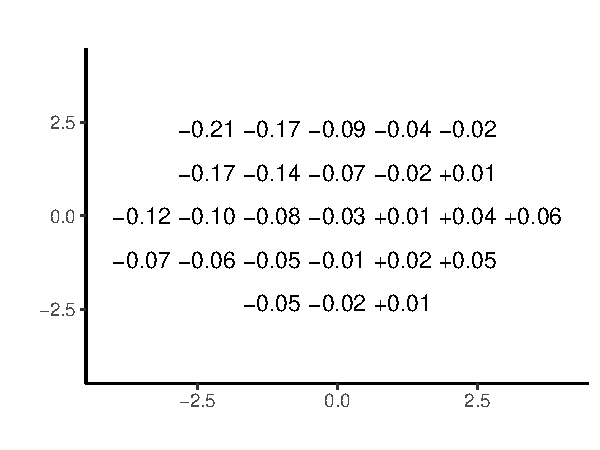
\includegraphics[width=0.31\linewidth]{rcode_and_data/figures/gaussian-example-plots-1} }
    \subfloat[$n = $ 500\label{fig:gaussian-example-plots2}]{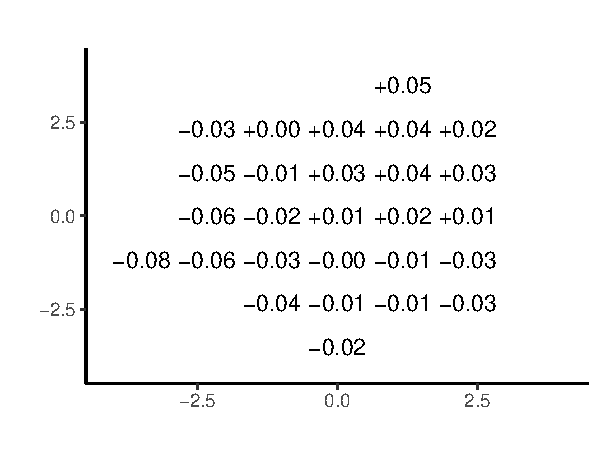
\includegraphics[width=0.31\linewidth]{rcode_and_data/figures/gaussian-example-plots-2} }
    \subfloat[$n = $ 2000\label{fig:gaussian-example-plots3}]{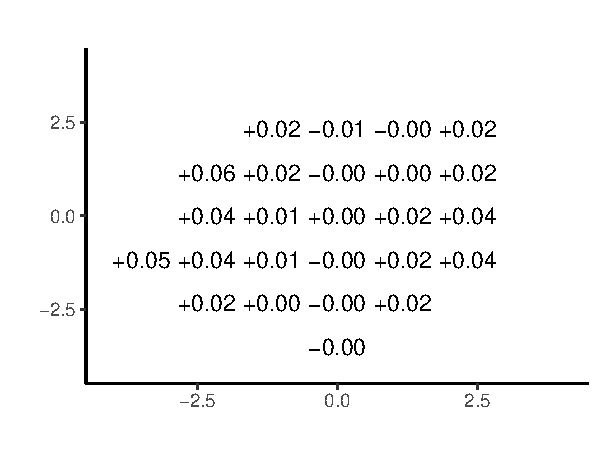
\includegraphics[width=0.31\linewidth]{rcode_and_data/figures/gaussian-example-plots-3} }
    \caption{Estimated local Gaussian partial correlation between $X_1$ and $X_2$ given $X_3 = 0$, where $(X_1, X_2, X_3)$ is a jointly standard normally distributed vector. The fully trivariate model of Section 3.1.1 is used.}\label{fig:gaussian-example-plots}
\end{figure}

In Figure \ref{fig:gaussian-example-plots} we see the estimated LGPC between \(X_1\) and \(X_2\) given \(X_3=0\) for three samples, having sample size 100, 500 and 2000 respectively, mapped out on a grid. In this and all other examples we select bandwidths based on a simple plug-in formula that follows naturally from classical asymptotic arguments, \(b = cn^{-1/9}\) for the full trivariate fit, and \(b = cn^{-1/6}\) for the bivariate simplification, where the constant \(c\) controls the amount of smoothing and must be chosen appropriately based on the task at hand. Otneim (\protect\hyperlink{ref-otneim2016multivariate}{2016}) argues that \(c=1.75\) is a good choice for multivariate density estimation, and we will in the next section see that we obtain good power in our test for conditional independence if \(c\) is somewhat smaller than that. For the visual display of conditional dependence maps, however, we tend to prefer a fair amount of smoothing, and in Figure \ref{fig:gaussian-example-plots} we have used \(c=4\). Otneim and Tjøstheim (\protect\hyperlink{ref-otneim2017locally}{2017}) also suggest an algorithm for bandwidth selection in the density estimation context, maximizing the leave-one-out cross validated log-likelihood of the sample;
\[\bb_{CV} = \textrm{arg max}_{\bb} \sum_{t = 1}^n \widehat{f}_{\bb}^{(-t)}(\Z_t),\]
where \(\widehat f_{\bb}^{(-t)}(\Z_t)\) is the estimated local Gaussian density estimate calculated without, and evaluated in, the sample point \(\Z_t\), using the bandwidth matrix \(\bb\). A theory of efficient and accurate bandwidth selection for local likelihood estimation remains a topic for future research.

As expected, \(\widehat\alpha(\x) = \widehat\alpha(\z)\) is close to zero in all three plots in Figure \ref{fig:gaussian-example-plots} and a significance test carried out as in Section \ref{chap:testing} does not reject conditional independence at any reasonable significance level.

\begin{figure}[p]
    \subfloat[Observed pairs $(X_1, X_2)$ from the conditionally \newline Gaussian model.\label{fig:simex2-plots1}]{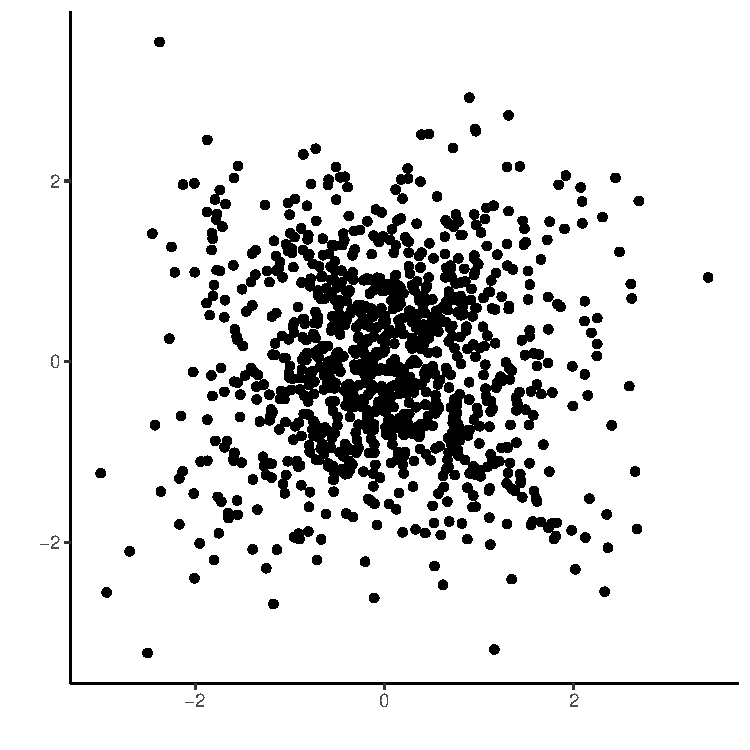
\includegraphics[width=0.49\linewidth]{rcode_and_data/figures/simex2-plots-1} }
    \subfloat[The estimated LGPC between $X_1$ and $X_2$ given $\rho = -0.9$.\label{fig:simex2-plots2}]{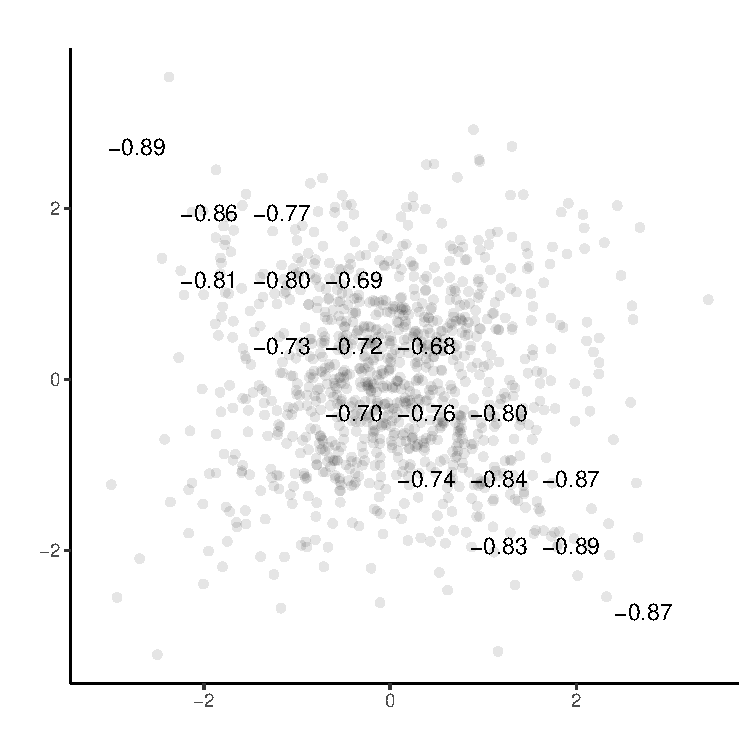
\includegraphics[width=0.49\linewidth]{rcode_and_data/figures/simex2-plots-2} }\newline
    \subfloat[The estimated LGPC between $X_1$ and $X_2$ \newline  given $\rho = 0$\label{fig:simex2-plots3}]{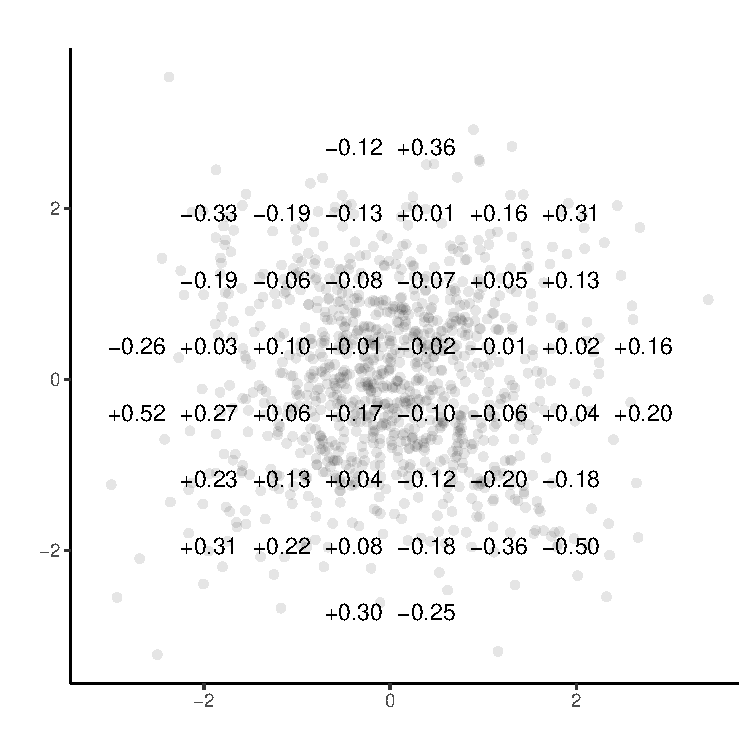
\includegraphics[width=0.49\linewidth]{rcode_and_data/figures/simex2-plots-3} }
    \subfloat[The estimated LGPC between $X_1$ and $X_2$ \newline given $\rho = 0.9$\label{fig:simex2-plots4}]{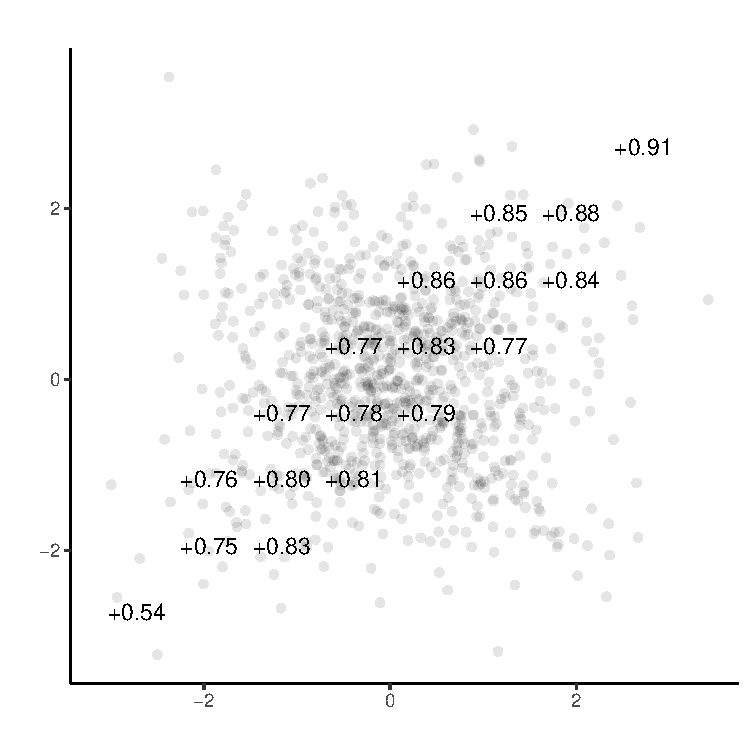
\includegraphics[width=0.49\linewidth]{rcode_and_data/figures/simex2-plots-4} }
    \caption{The conditionally Gaussian model}\label{fig:simex2-plots}
\end{figure}

In the next simulated example we will demonstrate an important feature of the LGPC: It is able to \emph{distinguish between positive and negative conditional relationships}, which, to our knowledge, has until now not been possible beyond the linear and jointly Gaussian setting using the ordinary partial correlation. Our approach also allows exploration of conditionally different dependence patterns across different levels of the conditioning variable.

Generate \(X_3 = \rho \sim U(-1,1)\), and then generate \((X_1, X_2)\) from the bivariate Gaussian distribution having standard normal marginals, and correlation coefficient equal to \(\rho\). We observe \(\X = (X_1, X_2, \rho)\) and seek to visualize the dependence between \(X_1\) and \(X_2\) conditional on \(\rho\).

We see the results in Figure \ref{fig:simex2-plots}. In panel (a), we display \(n=1000\) simulated pairs \((X_1, X_2)\) from this model. In panel (b)-(d) we see the estimated LGPC plotted over suitable grids, and where the conditioning variable \(X_3 = \rho\) has been fixed at the respective values \(-0.9\), \(0\) and \(0.9\), and we see clearly how the dependence between \(X_1\) and \(X_2\) dramatically changes in an intuitively reasonable way. By a conditioning argument one can see that \(X_1\) and \(X_2\) are uncorrelated and that the ordinary partial correlation between \(X_1\) and \(X_2\) given \(X_3\) is equal to zero. Furthermore, we note that the pairwise simplification defined in Section 3.1.2 would also not be able to measure the \emph{conditional} relationship between \(X_1\) and \(X_2\) given \(X_3\) in this case, as we see clearly from eq. \eqref{eq:scalardefinition}, because \(X_1\) and \(X_2\) are both marginally independent from \(X_3\). This means that the two pairwise correlations \(\rho_{13}(z_1,z_3)\) and \(\rho_{23}(z_2,z_3)\) are equal to zero.

We conclude this section by using the LGPC to analyze real data in an example regarding Granger causality between financial time series. Granger causality has been a central concept in economics and econometrics ever since its inception by Granger (\protect\hyperlink{ref-granger1969investigating}{1969}). In layman's terms, the time series \(\{X_t\}\) Granger causes \(\{Y_t\}\) if past values of \(\{X_t\}\) are helpful when predicting future values of \(\{Y_t\}\). Formally, \(\{X_t\}\) Granger causes \(\{Y_t\}\) if (Granger \protect\hyperlink{ref-granger1980testing}{1980})

\begin{equation}
Y_t \not\perp \mathcal{I}^*(t-1) \,\,|\,\, \mathcal{I}_{-X}^*(t-1),
\label{eq:granger}
\end{equation}
where \(\perp\) denotes independence, \(\not\perp\) denotes dependence, and where \(\mathcal{I}^*(t-1)\) is all information available at time \(t-1\) and \(\mathcal{I}_{-X}^*(t-1)\) is the same information, with the exception of the values of \(\{X_t\}\) up to, but not including, time \(t\). Of course, the hypothesis \eqref{eq:granger} can not be tested in practice in its full generality. By taking only effects up to the first lag into account, we may formulate a sufficient (but not necessary) condition for \eqref{eq:granger}: \(Y_t \not\perp X_{t-1} \,\,|\,\, Y_{t-1}\), the converse of which constitutes a testable null hypothesis of Granger non-causality:

\begin{equation}
\textrm{H}_0: Y_t \perp X_{t-1} \,\,|\,\, Y_{t-1}.
\label{eq:grangernull}
\end{equation}
There are many ways to carry out this test. The simplest, and original one, is based on the further restriction of linear relationships between \(\{X_t\}\) and \(\{Y_t\}\) and is thus a test for \emph{conditional uncorrelatedness} rather than conditional independence. Nonparametric tests that have power against many nonlinear types of conditional dependence have also been developed, and we refer to Section \ref{chap:testing} for further references to this literature and a new test for conditional independence based on the LGPC.

Francis, Mougoue, and Panchenko (\protect\hyperlink{ref-fran:moug:vale:2010}{2010}) investigate how stock returns of large firms may Granger cause the stock returns of small firms and vice versa from a nonlinear standpoint. They point to earlier evidence that such nonlinear lead-lag relationships have been found and investigate this further using the test for Granger non-causality by Baek and Brock (\protect\hyperlink{ref-baek:broc:1992}{1992}), and using a long series of US data they find evidence that there is a bi-directional causal link between the stock prices of the firms in the most valuable quintile (20 percent) and the firms in the least valuable quintile. We will repeat this exercise for stocks traded on the Oslo Stock Exchange in Norway, but this time from a point of view using the estimated LGPC.

Denote by \(R_{1,t}\) the log-returns on a value-weighted portfolio consisting of the most valuable quintile of firms listed on the Oslo Stock Exchange as of 27 April 2020 (the big firms), and denote by \(R_{2,t}\) the corresponding log-returns for the least valuable companies (the small firms). We will investigate the possibility of Granger causality from the small to the big firms, the hypothesis being that smaller firms are more market sensitive and quickly react to changes in the economy, leading the larger firms that more slowly adapt to small variations. The null hypothesis of non-causality of the first order \eqref{eq:grangernull} in this particular case means that

\begin{equation}
R_{1,t} \perp R_{2, t-1} \,\,|\,\, R_{1,t-1},
\end{equation}
which we may test formally using the approaches described in the following section or the references therein. Let us rather concentrate on \emph{describing} this conditional dependence relationship by estimating the local Gaussian partial correlation between \(R_{1,t}\) and \(R_{2,t-1}\) given a few different values of \(R_{2,t-1}\), which gives considerable more information than a single \(p\)-value of a test. We collect daily observations on Oslo Stock Exchange\footnote{Thanks to \emph{Børsprosjektet (The Stock Exchange Project)} at the Norwegian School of Economics for providing the data.} from 1 January 2018 until 31 December 2019. In Figure \ref{fig:order1} we see the estimated LGPC along the diagonal \(R_{1,t} = R_{2,t-1}\) for three different values \(R_{1,t-1} = -0.02, 0\) and \(0.02\), along with their block-bootstrapped 95\% confidence intervals. The constant \(\alpha(\z) = 0\) is indicated as a dotted line.

\begin{figure}[t]
\centering
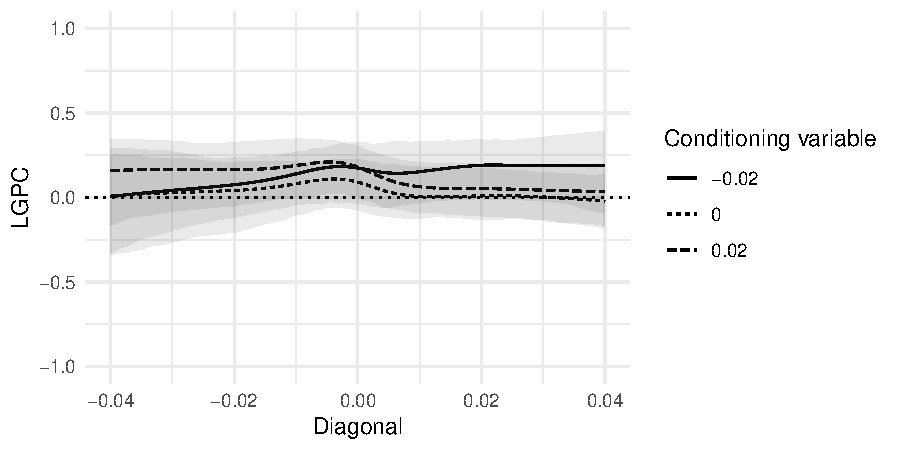
\includegraphics{rcode_and_data/figures/granger-order1}
\caption{The estimated LGPC between $R_{1,t}$ and $R_{2,t-1}$ given $R_{1,t-1}$ along the diagonal of the sample space, for three values of the conditioning variable}
\label{fig:order1}
\end{figure}

One could perhaps make the argument that \(R_{1,t}\) and \(R_{2,t-1}\) seem to be somewhat positively dependent in the right half of the graph for \emph{small} values of the conditioning variable \(R_{1,t-1}\). Roughly translated to this particular situation this means that if the large-firm portfolio gives a negative return on day \(t-1\), then its value on day \(t\) depend on the performance small-firm portfolio on day \(t-1\) in a nonlinear and non-Gaussian way that is characterized by positive dependence in the first quadrant. The evidence displayed in Figure \ref{fig:order1} is quite weak, however, because the confidence intervals include zero in most of the sample space.

Francis, Mougoue, and Panchenko (\protect\hyperlink{ref-fran:moug:vale:2010}{2010}) go on to analyze if there is Granger causality from small to big firms in the US data if another lag is taken into account, which in general means finding evidence against the hypothesis

\begin{equation}
R_{1,t} \perp (R_{2,t-1}, R_{2, t-2}) \,|\, (R_{1, t-1}, R_{1, t-2}),
\label{eq:order2}
\end{equation}
departures from which can be quantified and tested for in a linear fashion using multiple regressions, or tested for directly by means of a nonlinear test as we discuss in the following Section. Let us here, on the other hand, use the LGPC to quantify the conditional dependence relationship \eqref{eq:order2} nonlinearly for the Norwegian returns data in order to obtain more detailed information. This means estimating a \(3\times3\) partial correlation matrix \(\hfalpha(\z)\), which we again do along the diagonal \(R_{1,t} = R_{2,t-1} = R_{2, t-2}\) in this particular case.

\begin{figure}[t]
\centering
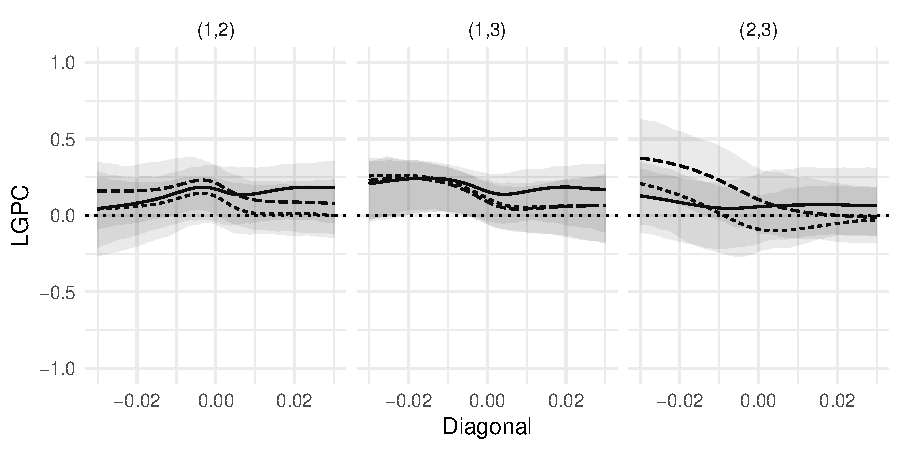
\includegraphics{rcode_and_data/figures/granger-order2}
\caption{The estimated local Gaussian partial correlations for the three variable pairs in $(R_{1,t}, R_{2,t-1}, R_{2, t-2})$ given $(R_{1, t-1}, R_{1, t-2})$ estimated along the diagonal in the sample space. The first two plots represent the pairs $(R_{1,t}, R_{2,t-1})$ and $(R_{1,t}, R_{2,t-2})$ which are of particular interest when analyzing the conditional dependence relationship \eqref{eq:order2}. The legend in Figure \ref{fig:order1} is still valid, except that the solid line now represents the LGPC conditional on \emph{both} $R_{1, t-1}$ and $R_{1, t-2}$ being equal to $-0.02$.}
\label{fig:order2}
\end{figure}

Including another lag does not change the estimated conditional relationship between \(R_{1,t}\) and \(R_{2,t-1}\) much compared to the first order estimate displayed in Figure \ref{fig:order1}. There does, however, seem to be a clearer picture when considering the LGPC between \(R_{1,t}\) and \(R_{2,t-2}\), which seems to be positive in the third quadrant for all values of the conditioning variables. In this particular problem this means that conditioning on the log return of the small-firm portfolio on days \(t-1\) and \(t-2\), the large-firm log-return on day \(t\) depends on the small-firm log-return on day \(t-2\) in a nonlinear way, and more specifically; this conditional relationship can be described using the LGPC as stronger dependence in the lower left tail of the relevant conditional distribution. We present another example of Granger testing in addition to another simulated experiment in Section J of the online supplement.

\hypertarget{chap:testing}{%
\section{TESTING FOR CONDITIONAL INDEPENDENCE}\label{chap:testing}}

We should point out here that the purpose of the LGPC is not primarily to compete with the nonparametric conditional independence \emph{testing} literature, but rather to provide a new tool for the measurement of nonlinear conditional dependence. The following section could however be seen as an indication of the potential of using the LGPC to test for conditional independence. It remains to be investigated whether further improvements can be realized by using a 5-parameter specification and/or a focused version of the test; see e.g.~Tables 3--5 of Lacal and Tjøstheim (\protect\hyperlink{ref-lacal2017local}{2017}) for the substantial improvements in a similar focused independence test.

We restrict ourselves to the case where \(X_1\) and \(X_2\) are scalars, since this is the situation considered in the papers we compare with, but we reiterate (end of Section \ref{chap:definition}) that there are no conceptual difficulties in extending to the vector case as is seen in the online supplement. The theory underlying LGPC testing is essentially based on Lacal and Tjøstheim (\protect\hyperlink{ref-lacal2018estimating}{2019}), and is outlined for the full vector case in Sections F--H of the supplement.

\hypertarget{fauna}{%
\subsection{The recent fauna of nonparametric tests}\label{fauna}}

Property 3 in Section \ref{properties} states that the LGPC characterizes conditional dependence within a quite large class of distributions: Two stochastic vectors \(X_1\) and \(X_2\) are independent given \(\X_3\) if and only if the locally Gaussian partial correlation between them is identically equal to zero everywhere on the sample space of \((X_1, X_2, \X_3)\). The road is therefore short to a test for conditional independence that may have power against a great deal of nonlinear alternatives compared to a test based on the ordinary partial correlation coefficient.

The last decade or so has seen the publication of many new tests for conditional independence. Su and White have published a series of such tests: Su and White (\protect\hyperlink{ref-su2007consistent}{2007}) is based on detecting differences between estimated characteristic functions (which is also the method used by Wang and Hong (\protect\hyperlink{ref-wang2017characteristic}{2018})). Su and White (\protect\hyperlink{ref-su2008nonparametric}{2008}) is based on estimating the Hellinger distance between conditional density estimates, Su and White (\protect\hyperlink{ref-su2012conditional}{2012}) use local polynomial quantile regression to test for conditional independence, and Su and White (\protect\hyperlink{ref-su2014testing}{2014}) present a test based on empirical likelihood. Huang (\protect\hyperlink{ref-huang2010testing}{2010}) introduces the maximal nonlinear conditional correlation which is used in a test for conditional independence, in turn extended to dependent data by Cheng and Huang (\protect\hyperlink{ref-cheng2012conditional}{2012}). Song (\protect\hyperlink{ref-song2009testing}{2009}) constructs a test via Rosenblatt transformations, while Bergsma (\protect\hyperlink{ref-bergsma2011nonparametric}{2010}) and Bouezmarni, Rombouts, and Taamouti (\protect\hyperlink{ref-bouezmarni2012nonparametric}{2012}) present new tests for conditional independence based on copula constructions. Bouezmarni and Taamouti (\protect\hyperlink{ref-boue:taam:2014}{2014}) test for conditional independence by measuring the \(L_2\) distance between estimated conditional distribution functions, and Patra, Sen, and Székely (\protect\hyperlink{ref-patra2016on}{2016}) use empirical transformations to translate conditional independence to joint independence, tests for which exist in abundance. Wang et al. (\protect\hyperlink{ref-wang2015conditional}{2015}) introduce the \emph{conditional distance correlation} which they use to construct a test for conditional independence. Linton and Gozalo (\protect\hyperlink{ref-linton1997conditional}{1997}, \protect\hyperlink{ref-linton2014testing}{2014}) formulate conditional independence in terms of probability statements which then forms the basis of a test. Also, Delgado and Manteiga (\protect\hyperlink{ref-delgado2001significance}{2001}) develop a test for conditional independence in a nonparametric regression framework. Finally, we mention testing by way of characterizing conditional independence via reproducing kernel Hilbert spaces (RKHS), see, for example, Zhang et al. (\protect\hyperlink{ref-zhang2012kernel}{2012}) and references therein.

A test based on the LGPC is quite different from the methods quoted above. It is semi-parametric and does not rely on traditional kernel estimates of density-, \mbox{distribution-,} or characteristic functions. Furthermore, due to our transformation of the data \eqref{eq:trans} to marginal standard normality, we do not necessarily have to specify weight functions in our test functional to lessen the impact of outliers - unless of course we wish to test for conditional independence in a specific portion of the sample space.

On the other hand, we have to pay a price when imposing structure on the dependence. Certain types of conditional dependence will remain invisible to our test statistic, but simulation experiments show that our test performs on par with, and sometimes better than existing, fully nonparametric tests.

\hypertarget{thetest}{%
\subsection{A test for conditional independence based on the LGPC}\label{thetest}}

We construct a test statistic for testing \(\textrm{H}_0: X_1 \perp X_2 \,\, | \,\, \X_3,\) or, equivalently, a test statistic in terms of the marginally Gaussian pseudo observations,

\begin{equation}
\textrm{H}_0: Z_1 \perp Z_2 \,\, | \,\, \Z_3,
\label{eq:ci-test}
\end{equation}
by aggregating our local measure of dependence over the sample space of \(\X\) (or \(\Z\)). A natural test statistic on the \(z\)-scale is

\begin{equation}
T_{n,b} = \int_S h\left( \widehat \alpha_b(\z)  \right) \di F_n(\z),
\label{eq:teststatistic}
\end{equation}
where \(h(\cdot)\) is a real-valued function that is typically even and non-negative for most standard applications, and \(S \subseteq \mathbb{R}^p\) is an integration area that can be altered in order to focus the test to specific portions of the sample space. Standard laws of large numbers ensure that, under regularity conditions, see Theorem F.1 of the supplement, \(T_{n,b}\) converges in probability towards its population value \[T = \int_S h\left(\alpha(\z)\right) \di F(\z).\]

Departures from conditional independence lead to large values of \(T_{n,b}\) that, if larger than a critical value, leads to the rejection of \eqref{eq:ci-test}. Asymptotically, one might expect that approximate \(p\)-values for our test can be extracted from the limiting distribution of the test statistic \(T_{n,b}\), which we derive in the online supplement Section F. The limiting asymptotic distribution of \(T_{n,b}-T\) is given in Theorem F.2 for the 1-parameter general pairwise case, whereas Theorem F.3 treats the 3-coordinate (3-parameter) case with \(d_1=d_2=d_3=1\). It is interesting to note from the discussion immediately following the proofs of these theorems that the convergence rate in the first case is \(n^{-1/2}\), and in the second case is \(\left(nb^2\right)^{-1/2}\). This means that the tests are asymptotically able to pick up alternatives approaching the null hypothesis of conditional independence at these rates. This is measured by the Pitman criterion. A discussion of the Pitman criterion for other tests of conditional independence is given on pages 11--12 immediately following Theorem 2 of Wang and Hong (\protect\hyperlink{ref-wang2017characteristic}{2018}). The rate \(n^{-1/2}b^{-d_3/4}\) of Wang and Hong compares favorable with other tests. The rate \(n^{-1/2}\) obtained by us must be interpreted with caution, however, because it is based on a pairwise model that is more restrictive. We go into more detail regarding local asymptotic power and the Pitman criterion in Section G of the online supplement.

Several authors, for example Teräsvirta, Tjøstheim, and Granger (\protect\hyperlink{ref-terasvirta2010modelling}{2010}), have noted, however, that asymptotic analysis of nonparametric (or semiparametric) test statistics on the form \eqref{eq:teststatistic} tends to be too crude for finite sample applications. We have therefore approximated the distribution of \(T_{n,b}\) using the bootstrap. The validity of the bootstrap in such contexts has been examined by Lacal and Tjøstheim (\protect\hyperlink{ref-lacal2018estimating}{2019}) and we adapt their arguments to our situation in the online supplement, Section H.

In accordance with our treatment so far, let \(\{Z_{1,t}, Z_{2, t}, \Z_{3, t}\}\), \(t = 1,\ldots,n\) be observations on the \(p\)-variate stochastic vector \(\Z\), \(p\geq3\), with \(Z_1\) and \(Z_2\) being scalar and \(\Z_3\) being \((p-2)\)-variate. In order to calculate the statistic \(T_{n,b}\) for testing the null hypothesis \(Z_1 \perp Z_2 \,\,|\,\, \Z_3\), we must estimate the joint local correlation matrix \(\fSigma(\z)\) of \(\Z = (Z_1, Z_2, \Z_3)\). We exploit this in the following algorithm designed to produce approximate resampled versions of \(T_{n,b}\) under the null hypothesis of conditional independence. This procedure is a variation of the so-called local bootstrap which has been used by several authors when testing for conditional independence. A brief survey of this procedure is given in Section I of the online supplement.

\begin{enumerate}
\def\labelenumi{\arabic{enumi}.}
\tightlist
\item
  Use the local correlation estimates to estimate the conditional densities \(f_{Z_1|\Z_3}(\cdot)\) and \(f_{Z_2|\Z_3}(\cdot)\) by means of the method by Otneim and Tjøstheim (\protect\hyperlink{ref-otneim2017conditional}{2018}). In practice, in order to reduce the computational load, we evaluate \(\widehat f_{Z_1|\Z_3}\) and \(\widehat f_{Z_2|\Z_3}\) on a fine grid on their support, over which a continuous representation of the estimates are produced using cubic splines.
\item
  Using the accept-reject algorithm, generate \(B\) samples, each of size \(n\), from \(\widehat f_{Z_1|\Z_3}\) and \(\widehat f_{Z_2|\Z_3}\), leading to \(B\) replicates
  \[Z_m^* = \Big\{\{Z_{1t}^*, Z_{2t}^*, \Z_{3t}^*\}_i\Big\}_m, \qquad t = 1,\ldots,n, \,\, m = 1,\ldots,B,\]
  of \(\Z\) under the null hypothesis.
\item
  Calculate \(\{T_{n,b}\}_m^*\), \(m = 1,\ldots,B\) for the replicated data sets and obtain the approximate \(p\)-value for the conditional independence test.
\end{enumerate}

\hypertarget{chap:testexamples}{%
\subsection{Comparing with other tests}\label{chap:testexamples}}

Su and White (\protect\hyperlink{ref-su2008nonparametric}{2008}) formulate a simulation experiment for evaluating their nonparametric test for conditional independence by generating data from 10 different data generating processes (DGPs), and then check the power and level for their test. Many of the later works that were discussed in Section \ref{fauna} contain very similar experiments, and some of them present simulation results for tests published prior to Su and White (\protect\hyperlink{ref-su2008nonparametric}{2008}). This allows us to present comprehensive comparisons between the new test presented above, and many alternatives.

Let \((\epsilon_{1,t}, \epsilon_{2,t}, \epsilon_{3,t})\) be IID observations from a \(\mathcal{N}(0, I_3)\)-distribution, where \(I_3\) is the \(3\times3\) identity matrix. We will test H\(_0: X_{1,t} \perp X_{2,t} \,\,|\,\, X_{3,t}\) in 10 cases listed in Table \ref{tab:dgps} taken from Su and White (\protect\hyperlink{ref-su2008nonparametric}{2008}), that cover various types of linear and nonlinear time series dependence.

\begin{table}[t]
\begin{tabular}{ll}
\hline
1.& $(X_{1,t}, X_{2,t}, X_{3,t}) = (\epsilon_{1,t}, \epsilon_{2,t}, \epsilon_{3,t})$.\\
2.& $X_{1,t} = 0.5X_{1, t-1} + \epsilon_{1,t}$, $X_{2,t} = 0.5X_{2,t-1} + \epsilon_{2,t}$, $X_{3,t} = X_{1,t-1}$.\\
3.& $X_{1,t} = \epsilon_{1,t}\sqrt{0.01 + 0.5X_ {1,t-1}^2}$, $X_{2,t} = 0.5X_{2, t-1} + \epsilon_{2,t}$, $X_{3,t} = X_{1,t-1}$.\\
4.& $X_{1,t} = \epsilon_{1,t}\sqrt{h_{1,t}}$, $X_{2,t} = \epsilon_{2,t}\sqrt{h_{2,t}}$, $X_{3,t} = X_{1,t-1}$, \\ & $h_{1,t}  = 0.01 + 0.9h_{1,t-1} + 0.05X_{1,t-1}^2$, $h_{2,t} = 0.01 + 0.9h_{2,t-1} + 0.05X_{2,t-1}^2$. \\
5.& $X_{1,t} = 0.5X_{1,t-1} + 0.5X_{2,t} + \epsilon_{1,t}$, $X_{2,t} = 0.5X_{2,t-1} + \epsilon_{2,t}$, $X_{3,t} = X_{1,t-1}$.\\
6.& $X_{1,t} = 0.5X_{1,t-1} + 0.5X_{2,t}^2 + \epsilon_{1,t}$, $X_{2,t} = 0.5X_{2,t-1} + \epsilon_{2,t}$, $X_{3,t} = X_{1,t-1}$.\\
7.& $X_{1,t} = 0.5X_{1,t-1}0.5X_{2,t} + \epsilon_{1,t}$, $X_{2,t} = 0.5X_{2,t-1} + \epsilon_{2,t}$, $X_{3,t} = X_{1,t-1}$.\\
8.& $X_{1,t} = 0.5X_{1,t-1} + 0.5X_{2,t}\epsilon_{1,t}$, $X_{2,t} = 0.5X_{2,t-1} + \epsilon_{2,t}$, $X_{3,t} = X_{1,t-1}$.\\
9.& $X_{1,t} = \epsilon_{1,t}\sqrt{0.01 + 0.5X_{1,t-1}^2 + 0.25X_{2,t}}$, $X_{2,t} = X_{2,t-1} + \epsilon_{2,t}$, $X_{3,t} = X_{1,t-1}$.\\
10. & $X_{1,t} = \epsilon_{1,t}\sqrt{h_{1,t}}$, $X_{2,t} = \epsilon_{2,t}\sqrt{h_{2,t}}$, $X_{3,t} = X_{1,t-1}$, $h_{1,t} = 0.01 + 0.1h_{1, t-1} + 0.4X_{1,t-1}^2 +$ \\ & $0.5X_{2,t}^2$, $h_{2,t} = 0.01 + 0.9h_{2, t-1} + 0.5X_t^2$.\\
\hline
\end{tabular}
\caption{Data generating processes in simulation experiment}
\label{tab:dgps}
\end{table}

The null hypotheses of conditional independence between \(X_{1,t}\) and \(X_{2,t}\) given \(X_{3,t}\) is true for DGPs 1--4, and these will be used to check the level of the test, while for DGPs 5--10 we measure the power. By evaluating our test using the sample sizes \(n = 100\) and \(n = 200\) at the \(5\%\) level, we can harvest a great number of corresponding results from the literature, and they are presented below.

The first set of simulation results are collected from Su and White (\protect\hyperlink{ref-su2008nonparametric}{2008}): In Table \ref{tab:n100} LIN is a standard linear Granger causality test, SCM and SKS are tests by Linton and Gozalo (\protect\hyperlink{ref-linton1997conditional}{1997}) that use statistics of the two versions of the nonparametric test developed by Delgado and Manteiga (\protect\hyperlink{ref-delgado2001significance}{2001}). HEL refers to the Hellinger distance test that Su and White (\protect\hyperlink{ref-su2008nonparametric}{2008}) present. Next, we move to Su and White (\protect\hyperlink{ref-su2014testing}{2014}), who provide simulations for their test for conditional independence based on the empirical likelihood (SEL), as well as the test by Su and White (\protect\hyperlink{ref-su2007consistent}{2007}) that is based on properties of the conditional characteristic function (CHF). Cheng and Huang (\protect\hyperlink{ref-cheng2012conditional}{2012}) provide simulations for their tests based on the maximal conditional correlation (MCC). In the online supplement to this article we provide a richer version of Table \ref{tab:n100}, namely Table 2*, that includes more results for the HEL- and MCC-tests at different levels of smoothing.



\renewcommand{\arraystretch}{1.2}
\begin{table}[t]
\resizebox{\textwidth}{!}{%
\begin{tabular}{l|rrrr|rrrrrr}
\toprule
&\multicolumn{4}{c}{Level} & \multicolumn{6}{c}{Power} \\
$\downarrow$ Test $\mid$ DGP $\rightarrow$ & 1 & 2 & 3 & 4 & 5 & 6 & 7 & 8 & 9 & 10 \\
\midrule
CHF&\texttt{0.034}&\texttt{0.058}&\texttt{-}&\texttt{-}&\texttt{0.780}&\texttt{0.792}&\texttt{0.520}&\texttt{0.780}&\texttt{0.728}&\texttt{0.580}\\
CM&\texttt{0.054}&\texttt{0.058}&\texttt{0.060}&\texttt{0.048}&\texttt{0.920}&\texttt{0.548}&\texttt{0.504}&\texttt{0.412}&\texttt{0.384}&\texttt{0.188}\\
HEL, $\scriptstyle c = 2$&\texttt{0.072}&\texttt{0.036}&\texttt{0.072}&\texttt{0.048}&\texttt{0.952}&\texttt{\underline{0.944}}&\texttt{0.576}&\texttt{0.940}&\texttt{\underline{0.988}}&\texttt{\underline{0.912}}\\
KS&\texttt{0.042}&\texttt{0.056}&\texttt{0.056}&\texttt{0.040}&\texttt{0.780}&\texttt{0.404}&\texttt{0.380}&\texttt{0.288}&\texttt{0.292}&\texttt{0.156}\\
\rowcolor{Gray}LGPC, $\scriptstyle c = 1.0$&\texttt{0.054}&\texttt{0.048}&\texttt{0.046}&\texttt{0.046}&\texttt{0.910}&\texttt{0.722}&\texttt{0.559}&\texttt{\underline{0.990}}&\texttt{0.968}&\texttt{0.866}\\
\rowcolor{Gray}LGPC, $\scriptstyle c = 1.4$&\texttt{0.047}&\texttt{0.043}&\texttt{0.046}&\texttt{0.047}&\texttt{0.971}&\texttt{0.855}&\texttt{0.727}&\texttt{0.969}&\texttt{0.916}&\texttt{0.765}\\
LIN&\texttt{0.044}&\texttt{0.061}&\texttt{0.050}&\texttt{0.060}&\texttt{\underline{0.999}}&\texttt{0.337}&\texttt{0.213}&\texttt{0.126}&\texttt{0.163}&\texttt{0.153}\\
MCC, $\scriptstyle c = 2$&\texttt{0.041}&\texttt{0.050}&\texttt{0.053}&\texttt{0.062}&\texttt{0.852}&\texttt{0.793}&\texttt{0.218}&\texttt{0.860}&\texttt{0.631}&\texttt{0.348}\\
SCM&\texttt{0.076}&\texttt{0.060}&\texttt{0.084}&\texttt{0.064}&\texttt{0.924}&\texttt{0.464}&\texttt{0.352}&\texttt{0.500}&\texttt{0.224}&\texttt{0.196}\\
SEL&\texttt{0.054}&\texttt{0.038}&\texttt{-}&\texttt{-}&\texttt{0.840}&\texttt{0.856}&\texttt{\underline{0.760}}&\texttt{0.904}&\texttt{0.716}&\texttt{0.556}\\
SKS&\texttt{0.064}&\texttt{0.056}&\texttt{0.088}&\texttt{0.068}&\texttt{0.728}&\texttt{0.236}&\texttt{0.288}&\texttt{0.340}&\texttt{0.120}&\texttt{0.112}\\
\bottomrule
\end{tabular}}
\caption{Level and power, $n = 100$}
\label{tab:n100}
\end{table}






Finally, we include results from simulations using our new test based on the LGPC, using the trivariate specification defined in Section \ref{chap:trivariate-full}, for two different levels of smoothing, and include them in Table \ref{tab:n100}. We highlight the new results in grey to indicate that they, as opposed to all the other numbers, have not appeared in the literature before. Also, to the best of our knowledge, these results have not been compared simultaneously before.

We see in Table \ref{tab:n100} that our test has the correct level and is quite powerful against all alternative specifications of conditional dependence, in the additive models 5 and 6, as well as the remaining examples 7 to 10, that are more multiplicative in nature.

When \(n=200\) we can include simulation results reported by Bouezmarni, Rombouts, and Taamouti (\protect\hyperlink{ref-bouezmarni2012nonparametric}{2012}) for their conditional independence test based on measuring the Hellinger distance between copula density estimates (shortened BRT from the names of the authors) as well as the results reported by Bouezmarni and Taamouti (\protect\hyperlink{ref-boue:taam:2014}{2014}) on their test based on \(L_2\) distances between estimated conditional distribution functions, which is abbreviated by BT. We include in Table 3* in the online supplement all results from these papers. The general picture is the same as in Table \ref{tab:n100}. In particular for the case with \(c=1.4\), our new test exhibits the best over-all performance among the examples listed, which, again to the best of our knowledge, include all such simulation results that have been published to date. It is seen that the standard linear Granger causality test (LIN) has a miserable performance in these examples.

Su and White (\protect\hyperlink{ref-su2014testing}{2014}) define two extensions to a subset of the data generating processes defined in Table 1 in which the conditioning variable \(\Xtwo\) is a vector with two and three components respectively. We refer to the online supplement for details regarding these extensions and numerical results. The new test for conditional independence based on the LGPC produces competitive results also in these cases. We point out again, however, that testing for conditional independence is merely one, albeit an important one, of several chief objectives for introducing the LGPC. Possible refinements of the LGPC testing is mentioned in the beginning of Section \ref{chap:testing}.

\hypertarget{conclusion-and-outlook}{%
\section{CONCLUSION AND OUTLOOK}\label{conclusion-and-outlook}}

The purpose of this paper is two-fold. First we define and develop the LGPC, a signed local measure of conditional dependence that has useful properties and is easy to interpret. It can measure both positive and negative conditional dependence. We then explore the possibility of using the LGPC in estimation of conditional dependence and indicate its potential in testing for conditional independence. The results are promising, and suggest that the newly developed tool provides powerful improvements to existing methods.

For 3 scalar variables \(X_1, X_2, X_3\) a full trivariate analysis depending on all 3 coordinates can be undertaken as in Section \ref{chap:trivariate-full}. If any of the components \(X_1, X_2\) or \(X_3\) are vectors, a pairwise approximation and simplification has been described in Section \ref{chap:bivariate} and in the supplement. This can be likened to additive approximation in nonparametric regression.

Both the full trivariate approach and the pairwise simplification have been mainly analyzed at the \(z\)-scale using the transformed variables \(\Z = \Phi^{-1}(F(\X))\). The corresponding LGPC \(\alpha(\z)\) is invariant to monotone transformations of the marginals. The LGPC \(\alpha(\x)\) on the \(x\)-scale can be obtained from \(\alpha(\z)\) by taking \(\x = F^{-1}(\Phi(\z))\), and it is in general different from \(\alpha(\z)\) and is not invariant to monotone transformations of the marginals. An analogue is the different transformation properties of the Pearson correlation and the copula structure in describing joint dependence. For multivariate Gaussian variables, \(\alpha(\x) \equiv \alpha(\z) \equiv \alpha\), which is the ordinary global partial correlation.

There is a potential for much further work. A next natural step may be structural equations as used in network analysis and Pearl-type causality (Pearl \protect\hyperlink{ref-pearl2000causality}{2000}), and ultimately further exploring the relationship or lack of relationship between that type of causality and Granger causality. All methods presented in this paper have been implemented in the R programming language (R Core Team \protect\hyperlink{ref-r}{2020}), and is available in the package \textbf{lg} (Otneim \protect\hyperlink{ref-otneim2019lg}{2019}). In addition, we provide code and data for easy replication of the results presented here in an online appendix.

\hypertarget{references}{%
\section*{REFERENCES}\label{references}}
\addcontentsline{toc}{section}{REFERENCES}

\hypertarget{refs}{}
\begin{cslreferences}
\leavevmode\hypertarget{ref-baba2004partial}{}%
Baba, Kunihiro, Ritei Shibata, and Masaaki Sibuya. 2004. ``Partial Correlation and Conditional Correlation as Measures of Conditional Independence.'' \emph{Australian \& New Zealand Journal of Statistics} 46 (4): 657--64.

\leavevmode\hypertarget{ref-baek:broc:1992}{}%
Baek, Ehung, and William Brock. 1992. ``A General Test for Nonlinear Granger Causality: Bivariate Model.'' \emph{Iowa State University and University of Wisconsin at Madison Working Paper}.

\leavevmode\hypertarget{ref-bergsma2011nonparametric}{}%
Bergsma, Wicher. 2010. ``Nonparametric Testing of Conditional Independence by Means of the Partial Copula.'' \emph{Unpublished Manuscript}. \url{http://dx.doi.org/10.2139/ssrn.1702981}.

\leavevmode\hypertarget{ref-bouezmarni2012nonparametric}{}%
Bouezmarni, Taoufik, Jeroen V K Rombouts, and Abderrahim Taamouti. 2012. ``Nonparametric Copula-Based Test for Conditional Independence with Applications to Granger Causality.'' \emph{Journal of Business and Economic Statistics} 30 (2): 275--87.

\leavevmode\hypertarget{ref-boue:taam:2014}{}%
Bouezmarni, Taoufik, and Abderrahim Taamouti. 2014. ``Nonparametric Tests for Conditional Independence Using Conditional Distributions.'' \emph{Journal of Nonparametric Statistics} 26 (4): 697--719.

\leavevmode\hypertarget{ref-cheng2012conditional}{}%
Cheng, Yu-Hsiang, and Tzee-Ming Huang. 2012. ``A Conditional Independence Test for Dependent Data Based on Maximal Conditional Correlation.'' \emph{Journal of Multivariate Analysis} 107: 210--26.

\leavevmode\hypertarget{ref-delgado2001significance}{}%
Delgado, Miguel A, and Wenceslao González Manteiga. 2001. ``Significance Testing in Nonparametric Regression Based on the Bootstrap.'' \emph{The Annals of Statistics} 29 (5): 1469--1507.

\leavevmode\hypertarget{ref-fran:moug:vale:2010}{}%
Francis, Bill B, Mbodja Mougoue, and Valentyn Panchenko. 2010. ``Is There a Symmetric Nonlinear Causal Relationship Between Large and Small Firms?'' \emph{Journal of Empirical Finance} 17 (1): 23--38.

\leavevmode\hypertarget{ref-granger1969investigating}{}%
Granger, Clive WJ. 1969. ``Investigating Causal Relations by Econometric Models and Cross-Spectral Methods.'' \emph{Econometrica}, 424--38.

\leavevmode\hypertarget{ref-granger1980testing}{}%
---------. 1980. ``Testing for Causality: A Personal Viewpoint.'' \emph{Journal of Economic Dynamics and Control} 2: 329--52.

\leavevmode\hypertarget{ref-hjort1996locally}{}%
Hjort, Nils Lid, and MC Jones. 1996. ``Locally Parametric Nonparametric Density Estimation.'' \emph{The Annals of Statistics}, 1619--47.

\leavevmode\hypertarget{ref-huang2010testing}{}%
Huang, Tzee-Ming. 2010. ``Testing Conditional Independence Using Maximal Nonlinear Conditional Correlation.'' \emph{The Annals of Statistics} 38 (4): 2047--91.

\leavevmode\hypertarget{ref-jordanger2017nonlinear}{}%
Jordanger, Lars Arne, and Dag Tjøstheim. 2020. ``Nonlinear Spectral Analysis: A Local Gaussian Approach.'' \emph{arXiv Preprint arXiv:1708.02166v4, Revised version submitted to the Journal of the American Statistical Association}.

\leavevmode\hypertarget{ref-lacal2017local}{}%
Lacal, Virginia, and Dag Tjøstheim. 2017. ``Local Gaussian Autocorrelation and Tests for Serial Independence.'' \emph{Journal of Time Series Analysis} 38 (1): 51--71.

\leavevmode\hypertarget{ref-lacal2018estimating}{}%
---------. 2019. ``Estimating and Testing Nonlinear Local Dependence Between Two Time Series.'' \emph{Journal of Business \& Economic Statistics} 37 (4): 648--60.

\leavevmode\hypertarget{ref-linton1997conditional}{}%
Linton, Oliver, and Pedro Gozalo. 1997. ``Conditional Independence Restrictions: Testing and Estimation.'' Unpublished manuscript.

\leavevmode\hypertarget{ref-linton2014testing}{}%
---------. 2014. ``Testing Conditional Independence Restrictions.'' \emph{Econometric Reviews} 33 (5-6): 523--52.

\leavevmode\hypertarget{ref-otneim2016multivariate}{}%
Otneim, Håkon. 2016. ``Multivariate and Conditional Density Estimation Using Local Gaussian Approximations.'' PhD thesis, University of Bergen; The University of Bergen.

\leavevmode\hypertarget{ref-otneim2019lg}{}%
Otneim, Håkon. 2019. \emph{\texttt{lg}: Locally Gaussian Distributions: Estimation and Methods}. \url{https://CRAN.R-project.org/package=lg}.

\leavevmode\hypertarget{ref-otneim2017locally}{}%
Otneim, Håkon, and Dag Tjøstheim. 2017. ``The Locally Gaussian Density Estimator for Multivariate Data.'' \emph{Statistics and Computing} 27 (6): 1595--1616.

\leavevmode\hypertarget{ref-otneim2017conditional}{}%
---------. 2018. ``Conditional Density Estimation Using the Local Gaussian Correlation.'' \emph{Statistics and Computing} 28 (2): 303--21.

\leavevmode\hypertarget{ref-patra2016on}{}%
Patra, Rohit K, Bodhisattva Sen, and Gábor J Székely. 2016. ``On a Nonparametric Notion of Residual and Its Applications.'' \emph{Statistics and Probability Letters} 109: 208--13.

\leavevmode\hypertarget{ref-pearl2000causality}{}%
Pearl, Judea. 2000. \emph{Causality: Models, Reasoning and Inference}. Vol. 29. Springer.

\leavevmode\hypertarget{ref-r}{}%
R Core Team. 2020. \emph{R: A Language and Environment for Statistical Computing}. Vienna, Austria: R Foundation for Statistical Computing. \url{https://www.R-project.org/}.

\leavevmode\hypertarget{ref-song2009testing}{}%
Song, Kyungchul. 2009. ``Testing Conditional Independence via Rosenblatt Transforms.'' \emph{The Annals of Statistics} 37 (6B): 4011--45.

\leavevmode\hypertarget{ref-su2007consistent}{}%
Su, Liangjun, and Halbert White. 2007. ``A Consistent Characteristic Function-Based Test for Conditional Independence.'' \emph{Journal of Econometrics} 141 (2): 807--34.

\leavevmode\hypertarget{ref-su2008nonparametric}{}%
---------. 2008. ``A Nonparametric Hellinger Metric Test for Conditional Independence.'' \emph{Econometric Theory} 24 (4): 829--64.

\leavevmode\hypertarget{ref-su2014testing}{}%
---------. 2014. ``Testing Conditional Independence via Empirical Likelihood.'' \emph{Journal of Econometrics} 182 (1): 27--44.

\leavevmode\hypertarget{ref-su2012conditional}{}%
Su, Liangjun, and Halbert L White. 2012. ``Conditional Independence Specification Testing for Dependent Processes with Local Polynomial Quantile Regression.'' In \emph{Essays in Honor of Jerry Hausman}, 355--434. Emerald Group Publishing Limited.

\leavevmode\hypertarget{ref-terasvirta2010modelling}{}%
Teräsvirta, Timo, Dag Tjøstheim, and Clive W. J. Granger. 2010. \emph{Modelling Nonlinear Economic Time Series}. Oxford University Press.

\leavevmode\hypertarget{ref-tjostheim2013local}{}%
Tjøstheim, Dag, and Karl Ove Hufthammer. 2013. ``Local Gaussian Correlation: A New Measure of Dependence.'' \emph{Journal of Econometrics} 172 (1): 33--48.

\leavevmode\hypertarget{ref-wang2017characteristic}{}%
Wang, Xia, and Yongmiao Hong. 2018. ``Characteristic Function Based Testing for Conditional Independence: A Nonparametric Regression Approach.'' \emph{Econometric Theory} 34 (4): 815--49.

\leavevmode\hypertarget{ref-wang2015conditional}{}%
Wang, Xueqin, Wenliang Pan, Wenhao Hu, Yuan Tian, and Heping Zhang. 2015. ``Conditional Distance Correlation.'' \emph{Journal of the American Statistical Association} 110 (512): 1726--34.

\leavevmode\hypertarget{ref-zhang2012kernel}{}%
Zhang, Kun, Jonas Peters, Dominik Janzing, and Bernhard Schölkopf. 2012. ``Kernel-Based Conditional Independence Test and Application in Causal Discovery.'' \emph{arXiv Preprint arXiv:1202.3775}.
\end{cslreferences}

\end{document}
